\documentclass[]{krantz}
\usepackage{lmodern}
\usepackage{amssymb,amsmath}
\usepackage{ifxetex,ifluatex}
\usepackage{fixltx2e} % provides \textsubscript
\ifnum 0\ifxetex 1\fi\ifluatex 1\fi=0 % if pdftex
  \usepackage[T1]{fontenc}
  \usepackage[utf8]{inputenc}
\else % if luatex or xelatex
  \ifxetex
    \usepackage{mathspec}
  \else
    \usepackage{fontspec}
  \fi
  \defaultfontfeatures{Ligatures=TeX,Scale=MatchLowercase}
\fi
% use upquote if available, for straight quotes in verbatim environments
\IfFileExists{upquote.sty}{\usepackage{upquote}}{}
% use microtype if available
\IfFileExists{microtype.sty}{%
\usepackage[]{microtype}
\UseMicrotypeSet[protrusion]{basicmath} % disable protrusion for tt fonts
}{}
\PassOptionsToPackage{hyphens}{url} % url is loaded by hyperref
\usepackage[unicode=true]{hyperref}
\PassOptionsToPackage{usenames,dvipsnames}{color} % color is loaded by hyperref
\hypersetup{
            pdftitle={Advanced Big Data Analytics for Business with R},
            pdfauthor={Sanjeev Kumar},
            colorlinks=true,
            linkcolor=Maroon,
            citecolor=Blue,
            urlcolor=Blue,
            breaklinks=true}
\urlstyle{same}  % don't use monospace font for urls
\usepackage{natbib}
\bibliographystyle{apalike}
\usepackage{color}
\usepackage{fancyvrb}
\newcommand{\VerbBar}{|}
\newcommand{\VERB}{\Verb[commandchars=\\\{\}]}
\DefineVerbatimEnvironment{Highlighting}{Verbatim}{commandchars=\\\{\}}
% Add ',fontsize=\small' for more characters per line
\usepackage{framed}
\definecolor{shadecolor}{RGB}{248,248,248}
\newenvironment{Shaded}{\begin{snugshade}}{\end{snugshade}}
\newcommand{\KeywordTok}[1]{\textcolor[rgb]{0.27,0.27,0.27}{\textbf{#1}}}
\newcommand{\DataTypeTok}[1]{\textcolor[rgb]{0.27,0.27,0.27}{#1}}
\newcommand{\DecValTok}[1]{\textcolor[rgb]{0.06,0.06,0.06}{#1}}
\newcommand{\BaseNTok}[1]{\textcolor[rgb]{0.06,0.06,0.06}{#1}}
\newcommand{\FloatTok}[1]{\textcolor[rgb]{0.06,0.06,0.06}{#1}}
\newcommand{\ConstantTok}[1]{\textcolor[rgb]{0,0,0}{#1}}
\newcommand{\CharTok}[1]{\textcolor[rgb]{0.5,0.5,0.5}{#1}}
\newcommand{\SpecialCharTok}[1]{\textcolor[rgb]{0,0,0}{#1}}
\newcommand{\StringTok}[1]{\textcolor[rgb]{0.5,0.5,0.5}{#1}}
\newcommand{\VerbatimStringTok}[1]{\textcolor[rgb]{0.5,0.5,0.5}{#1}}
\newcommand{\SpecialStringTok}[1]{\textcolor[rgb]{0.5,0.5,0.5}{#1}}
\newcommand{\ImportTok}[1]{#1}
\newcommand{\CommentTok}[1]{\textcolor[rgb]{0.56,0.35,0.01}{\textit{#1}}}
\newcommand{\DocumentationTok}[1]{\textcolor[rgb]{0.56,0.35,0.01}{\textbf{\textit{#1}}}}
\newcommand{\AnnotationTok}[1]{\textcolor[rgb]{0.56,0.35,0.01}{\textbf{\textit{#1}}}}
\newcommand{\CommentVarTok}[1]{\textcolor[rgb]{0.56,0.35,0.01}{\textbf{\textit{#1}}}}
\newcommand{\OtherTok}[1]{\textcolor[rgb]{0.56,0.35,0.01}{#1}}
\newcommand{\FunctionTok}[1]{\textcolor[rgb]{0.00,0.00,0.00}{#1}}
\newcommand{\VariableTok}[1]{\textcolor[rgb]{0.00,0.00,0.00}{#1}}
\newcommand{\ControlFlowTok}[1]{\textcolor[rgb]{0.13,0.29,0.53}{\textbf{#1}}}
\newcommand{\OperatorTok}[1]{\textcolor[rgb]{0.81,0.36,0.00}{\textbf{#1}}}
\newcommand{\BuiltInTok}[1]{#1}
\newcommand{\ExtensionTok}[1]{#1}
\newcommand{\PreprocessorTok}[1]{\textcolor[rgb]{0.56,0.35,0.01}{\textit{#1}}}
\newcommand{\AttributeTok}[1]{\textcolor[rgb]{0.77,0.63,0.00}{#1}}
\newcommand{\RegionMarkerTok}[1]{#1}
\newcommand{\InformationTok}[1]{\textcolor[rgb]{0.56,0.35,0.01}{\textbf{\textit{#1}}}}
\newcommand{\WarningTok}[1]{\textcolor[rgb]{0.56,0.35,0.01}{\textbf{\textit{#1}}}}
\newcommand{\AlertTok}[1]{\textcolor[rgb]{0.94,0.16,0.16}{#1}}
\newcommand{\ErrorTok}[1]{\textcolor[rgb]{0.64,0.00,0.00}{\textbf{#1}}}
\newcommand{\NormalTok}[1]{#1}
\usepackage{longtable,booktabs}
% Fix footnotes in tables (requires footnote package)
\IfFileExists{footnote.sty}{\usepackage{footnote}\makesavenoteenv{long table}}{}
\usepackage{graphicx,grffile}
\makeatletter
\def\maxwidth{\ifdim\Gin@nat@width>\linewidth\linewidth\else\Gin@nat@width\fi}
\def\maxheight{\ifdim\Gin@nat@height>\textheight\textheight\else\Gin@nat@height\fi}
\makeatother
% Scale images if necessary, so that they will not overflow the page
% margins by default, and it is still possible to overwrite the defaults
% using explicit options in \includegraphics[width, height, ...]{}
\setkeys{Gin}{width=\maxwidth,height=\maxheight,keepaspectratio}
\IfFileExists{parskip.sty}{%
\usepackage{parskip}
}{% else
\setlength{\parindent}{0pt}
\setlength{\parskip}{6pt plus 2pt minus 1pt}
}
\setlength{\emergencystretch}{3em}  % prevent overfull lines
\providecommand{\tightlist}{%
  \setlength{\itemsep}{0pt}\setlength{\parskip}{0pt}}
\setcounter{secnumdepth}{5}
% Redefines (sub)paragraphs to behave more like sections
\ifx\paragraph\undefined\else
\let\oldparagraph\paragraph
\renewcommand{\paragraph}[1]{\oldparagraph{#1}\mbox{}}
\fi
\ifx\subparagraph\undefined\else
\let\oldsubparagraph\subparagraph
\renewcommand{\subparagraph}[1]{\oldsubparagraph{#1}\mbox{}}
\fi

% set default figure placement to htbp
\makeatletter
\def\fps@figure{htbp}
\makeatother

\usepackage{booktabs}
\usepackage{longtable}
\usepackage[bf,singlelinecheck=off]{caption}

\usepackage{framed,color}
\definecolor{shadecolor}{RGB}{248,248,248}

\renewcommand{\textfraction}{0.05}
\renewcommand{\topfraction}{0.8}
\renewcommand{\bottomfraction}{0.8}
\renewcommand{\floatpagefraction}{0.75}

\renewenvironment{quote}{\begin{VF}}{\end{VF}}
\let\oldhref\href
\renewcommand{\href}[2]{#2\footnote{\url{#1}}}

\makeatletter
\newenvironment{kframe}{%
\medskip{}
\setlength{\fboxsep}{.8em}
 \def\at@end@of@kframe{}%
 \ifinner\ifhmode%
  \def\at@end@of@kframe{\end{minipage}}%
  \begin{minipage}{\columnwidth}%
 \fi\fi%
 \def\FrameCommand##1{\hskip\@totalleftmargin \hskip-\fboxsep
 \colorbox{shadecolor}{##1}\hskip-\fboxsep
     % There is no \\@totalrightmargin, so:
     \hskip-\linewidth \hskip-\@totalleftmargin \hskip\columnwidth}%
 \MakeFramed {\advance\hsize-\width
   \@totalleftmargin\z@ \linewidth\hsize
   \@setminipage}}%
 {\par\unskip\endMakeFramed%
 \at@end@of@kframe}
\makeatother

\renewenvironment{Shaded}{\begin{kframe}}{\end{kframe}}

\usepackage{makeidx}
\makeindex
\renewcommand{\indexname}{Index of R Commands, Packages and Key Concepts}
\usepackage[columns=3]{idxlayout}


% \newcommand\rcommand[1]{
% \colorbox{yellow}{\texttt{\color{red} #1}}
% %\sidebar{\textbf{\color{red} #1 \\}}
% \index{R Commands!#1}
% }

\urlstyle{tt}

\usepackage{amsthm}
\makeatletter
\def\thm@space@setup{%
  \thm@preskip=8pt plus 2pt minus 4pt
  \thm@postskip=\thm@preskip
}
\makeatother

\frontmatter

\title{Advanced Big Data Analytics for Business with R}
\author{Sanjeev Kumar}
\date{2018-12-19}

\usepackage{amsthm}
\newtheorem{theorem}{Theorem}[chapter]
\newtheorem{lemma}{Lemma}[chapter]
\theoremstyle{definition}
\newtheorem{definition}{Definition}[chapter]
\newtheorem{corollary}{Corollary}[chapter]
\newtheorem{proposition}{Proposition}[chapter]
\theoremstyle{definition}
\newtheorem{example}{Example}[chapter]
\theoremstyle{definition}
\newtheorem{exercise}{Exercise}[chapter]
\theoremstyle{remark}
\newtheorem*{remark}{Remark}
\newtheorem*{solution}{Solution}
\let\BeginKnitrBlock\begin \let\EndKnitrBlock\end
\begin{document}
\maketitle

% you may need to leave a few empty pages before the dedication page

%\cleardoublepage\newpage\thispagestyle{empty}\null
%\cleardoublepage\newpage\thispagestyle{empty}\null
%\cleardoublepage\newpage
\thispagestyle{empty}

\begin{center}

\par\vspace*{.35\textheight}{\centering \texttt{dedicated to the one to whom I owe all} \par}

%\includegraphics{images/dedication.pdf}
\end{center}

\setlength{\abovedisplayskip}{-5pt}
\setlength{\abovedisplayshortskip}{-5pt}

{
\hypersetup{linkcolor=black}
\setcounter{tocdepth}{2}
\tableofcontents
}
\listoftables
\listoffigures
\chapter*{Go Blue!}\label{go-blue}


\begin{figure}
\centering
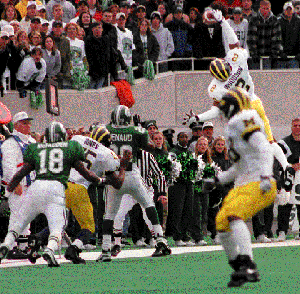
\includegraphics{images/woodson.png}
\caption{}
\end{figure}

\begin{quote}
Until I build a cover image for this book, Woodson's Giant Leap will
have to suffice.
\end{quote}

\chapter*{Preface}\label{preface}


We live in a world awash in data. Companies are increasingly turning to
data analytics to extract a competitive edge from data, especially
large, complex datasets often called \emph{Big Data}. However, companies
are increasingly facing the challenge posed by the scarcity of
analytical talent - people who can turn data into better decisions,
people who can extract insights and information from data. There is
growing demand for professionals with strong quantitative skills
combined with an understanding of how data analytic techniques can be
applied to business contexts and managerial decision making. To help my
students succeed in this growing field, I teach classes in
\textbf{Advanced Big Data Analytics} in Ross School of Business, Univ.
of Michigan. In these courses I teache advanced analytical, statistical
and data mining tools with an applied focus. This book is developed
specifically for these courses.

The main focus of this book (and the associated coures) is to prepare
students to model and manage business decisions with data analytics and
decision models using real life case contexts and datasets. By the end
of this book students will have a better understanding of processes,
methodologies and tools used to transform the large amount of business
data available into useful information and support business decision
making. The book will focus on extracting actionable business
intelligence by analyzing traditional business data as well as more
recently available datasets such as social media, crowdsourcing and
recommendation engines. The book focuses on the powerful, open source
(and hence free) data analysis environment R.

As I designed these courses, I realized that while there are a lot of
references available for doing Advanced Analytics on Big Data using R,
there isn't a good reference that approaches the topic from the
perspective of business students and is accessible for students who do
not have extensive background in statistics or computer programming. I
designed my classes to have an applied nature with significant amount of
hands-on work on real business Big Data with significant managerial
implications. I emphasized aspects of the analytics process that are
important for actual practice of data science but are not typically well
covered in traditonal textbooks - like data cleaning, managing large
datasets and building data dashboards. I ended up creating a significant
amount of material for the classes - much of it collated from already
available but widely dispersed sources. This book is a collection of
these material.

Business students have a unique mixture of tech savvy, super smarts and
learning ability with a relative lack of computer programming or coding
experience. They further have a great applied sense of statistics and
data analysis but typically without the theoretical expertise of a
Statistics student. This book is directed towards such students. This
book assumes that business students are joining an Advanced Analytics
course without any knowledge of computer programming and without any
background in R. This book assumes that students are familiar with basic
probability and statistics but their focus is on applied statistics -
not on the theory. The book then builds up student's comfort level with
R while at the same time makeing progress on key Advanced Analytics
materials.

Direct all feedback on this book to the author at
email:\texttt{sankum\ at\ umich.edu} or twitter: \texttt{@a\_teachr}.

\section*{Who Is This Book For?}\label{who-is-this-book-for}


This book is for business students, practitioners and executives who
want to have hands-on experience in working with business related big
data and want to extract actionable insights from the data using
advanced analytical techniques. This book is application oriented and
hence focuses on the application of advanced analytical techniques
rather than the theoretical details. Consequently, this book is not for
readers solely focused on the theoretical, statistical part of data
analytics.

This book assumes that the readers have basic familiarity with
introductory probability and statistics. This domain is easier to follow
and understand if the reader also has \emph{some} exposure to
\emph{some} kind of computer programming although that is not a
necessity. This book has been written for a practitioner audience, not
an academic one. The book aims to be an exhaustive reference resource
for practitioners - that's why it starts with baby steps of introducing
R and basic data manipulation and ends at the other end with advanced
Machine Learning algorithms and complex model improvement algorithms.

Thank you for placing your trust in this book. This chapter will
provider further details about this book and how to best read/use this
book.

\section*{About This Document}\label{about-this-document}


This document, which you are probably seeing as a GitHub eBook or a PDF
document or even as printed book, has been written entirely using R and
RStudio. This book is built using the \textbf{knitr}\index{knitr}
package \citep{xie2015} and the \textbf{bookdown}\index{bookdown}
package \citep{R-bookdown}. PDF version of the book is created using my
favorite document creation system called \textbf{LaTeX}. This document
has been created entirely using Open Source tools and has been released
back into the Open Source ecosystem for free using the GNU General
Public License (GPL). You are free to share this document with others as
long as you comply with the GPL license. GPL License usually require
that the product (in this case, this book) be made available free or
charge; and any subsequent product made using the GPL Licensed product
must also be made available free of charge \citep{TheGNUGe51:online}.

This is my first attempt at writing a book size document. I have had to
develop a bunch of workarounds to make the process work and get a
quality output. The source code for this book is available for public
use free of charge at: \url{https://github.com/clarifyR/AABookDown}. The
HTML and PDF versions are available (again, free of charge) at:
\url{http://clarifyr.com/AABookDown/}. This book is a live document
which is continually updated as I teach my classes and learn more about
student needs. A printed version will be available for purchase from
Amazon once the book is substantially complete.

Following is the R session information that built the current version:

\begin{Shaded}
\begin{Highlighting}[]
\NormalTok{xfun}\OperatorTok{::}\KeywordTok{session_info}\NormalTok{()}
\end{Highlighting}
\end{Shaded}

\begin{verbatim}
## R version 3.4.3 (2017-11-30)
## Platform: x86_64-apple-darwin15.6.0 (64-bit)
## Running under: macOS  10.14.1
## 
## Locale: en_US.UTF-8 / en_US.UTF-8 / en_US.UTF-8 / C / en_US.UTF-8 / en_US.UTF-8
## 
## Package version:
##   backports_1.1.2 base64enc_0.1.3 bookdown_0.5   
##   compiler_3.4.3  digest_0.6.13   evaluate_0.10.1
##   graphics_3.4.3  grDevices_3.4.3 highr_0.6      
##   htmltools_0.3.6 jsonlite_1.5    knitr_1.18     
##   magrittr_1.5    markdown_0.8    methods_3.4.3  
##   mime_0.5        Rcpp_0.12.14    rmarkdown_1.8  
##   rprojroot_1.3-2 rstudioapi_0.7  stats_3.4.3    
##   stringi_1.1.6   stringr_1.2.0   tools_3.4.3    
##   utils_3.4.3     xfun_0.3        yaml_2.1.19
\end{verbatim}

\section*{How is This Book
Structured}\label{how-is-this-book-structured}


This book covers a wide range of material. The material is organized in
5 parts, 19 chapters and several appendices.

\subsection*{Part I: Getting Started}\label{part-i-getting-started}


We set ourselves for the book - download and install all needed
software; figure our way around R and RStudio and learn the basics of
the R language. Essentially lay down enough of a foundation that we can
start getting productive. For students without a computer programming
background, it is essential that they do not rush this part. Our success
in later parts depend upon us getting comfortable with the material
here.

\subsection*{Part II: Data Exploration and
Visualization}\label{part-ii-data-exploration-and-visualization}
\addcontentsline{toc}{subsection}{Part II: Data Exploration and
Visualization}

Real data analytics begins with us understanding and getting a handle on
the data. This typically involves cleaning up the data, generating
descriptive statistics to better understand the data and finally
creating visualizations that allow us to better understand the
underlying complexity of the data. In my opinion, data cleaning is the
most under-appreciated part of data analytics. It often takes more time
and effort than the actual analysis that follows.

Data visualization has emerged as a key tool in Big Data Analytics. We
specifically focus our attention here on a subset of data visualization
that is important in the business context - creating data dashboards
that can help managerial decision making.

\subsection*{Part III: Traditional Statistical
Modeling}\label{part-iii-traditional-statistical-modeling}
\addcontentsline{toc}{subsection}{Part III: Traditional Statistical
Modeling}

Even advanced analytic techniques like machine learning algorithms in
the next part have their foundations in traditional statistical
methodologies. Classical statistical modeling approaches like Linear
Regression are still the benchmark given their immense popularity,
flexibility and stability. In this part of the book, we explore
traditional statistical analysis tools like Linear Regression,
Generalized Linear Models like Logistic and Survival Models, Principal
Components and Factor Analysis, Time Series Analysis and so on.

As we assume that you are already familiar with basic probability and
statistics, we will focus on application of the methodologies and not
the underlying theory. We will also focus on how to tweak these tools
for the Big Data world as many of these tools run into trouble when
sample sizes are quite large. Bigger is not always better - traditional
statisticall methodologies were developed/optimized for smaller sample
sizes. Using them for large sample sizes give rise to unique issues and
problems - we will discuss how to address them.

\subsection*{Part IV: Machine Learning and Predictive
Analytics}\label{part-iv-machine-learning-and-predictive-analytics}
\addcontentsline{toc}{subsection}{Part IV: Machine Learning and
Predictive Analytics}

This is the largest and the most important part of the book. This is why
this book was written in the first place - an overview of data analytics
tools specific to Big Data - variously known as Machine Learning,
Statistical Learning, Predictive Analytics, Data Mining as so on. This
book focuses on tools that help us make sense of Big Data and helps us
automate the extraction of managerial decision making insights from Big
Data.

As with much of the rest of the book, the focus is on applying the tools
rather than their theoretical/mathematical underpinnings. We will
discuss enough theory to develop an overall understanding and then
devote our energies on making these tools work on real datasets.

\subsection*{Part V: Putting It All
Together}\label{part-v-putting-it-all-together}


Now that we have gone through all the elements individually, we can move
forward to create a combined, integrated approach that puts all these
pieces together. How to combine different models so that they result in
an output better than sum of their parts? How to ensure that our models
improve as more data become available?

\subsection*{Part VI: Appendices, Bibliography and
Index}\label{part-vi-appendices-bibliography-and-index}
\addcontentsline{toc}{subsection}{Part VI: Appendices, Bibliography and
Index}

Back matter of the book. The Index in the end has three main components
- Key Concepts, R Commands and R Packages. Appendices include syllabus
for the courses this book is primarily used for and other miscellaneous
content that did not fit in one of the main matter chapters. The index
is only available in the PDF format of the book.

There are a lot of quality, free, online resources available for
building up your R and Data Analytics skills before you go through this
book or the associated courses. They are listed in Appendix: Key
References. A fully fleshed data analysis example has been presented on
Appendix: Data Analysis Example to give you an idea of the power and
range of what can be accomplished with just a little bit of familiarity
with R.

\section*{How to Read This Book}\label{how-to-read-this-book}


You would have noticed by now that this book integrates R code within
its text. Most of the time R code takes the form of dedicated code
blocks like the one below:

\begin{Shaded}
\begin{Highlighting}[]
\CommentTok{#This is a demo code block}
\KeywordTok{print}\NormalTok{(}\StringTok{"Hello World"}\NormalTok{)}
\end{Highlighting}
\end{Shaded}

\begin{verbatim}
## [1] "Hello World"
\end{verbatim}

As you can see from above, code blocks are printed in color, in
\texttt{fixed\ width\ font}. There is a color scheme here that you will
soon become familiar with - comments, functions, strings all haver their
specific formatting. The output of the code block appears right after -
for example - the output of the \textbf{\texttt{print()}} command
follows the code above.

You would notice that whenever we refer to a R command in a significant
way (like \textbf{\texttt{print()}} in paragraph above), the command is
printed in \texttt{fixed\ width\ font}, in bold that makes it easy for
you to see which commands are discussed significantly on the page. The
highlighting also ensures that an entry for the command is placed in the
Index provided at the end of the book. For times when a command is
mentioned in text in a minor way not necessating an Index entry, they
will be typed in \texttt{fixed\ width\ font}.

Like R Commands, this book provides special formatting for R Packages
used in the book. R Packages are fomatted like R Commands with an entry
in the Packages section of the Index. Lastly, special formatting is
provided for key concepts - similar to R Commands and Packages and their
Index entry is in the Key Concepts section. For example: this book
focuses on \textbf{\texttt{Open\ Source}} software - that are created by
a community of software developers for use by the community, usually
made available for free.

The three special formatting elements - commands, packages and key
concepts - ensure that you have a summary of significant elements
discussed in the page just by looking for highlighted items.

\section*{Is This Book Suitable For
You?}\label{is-this-book-suitable-for-you}


Well - you wouldn't know until you spend some time with it. Dig in.

A quick word of caution though before you get too deep: this book (and
the associated courses) are very hands-on. There is no point in reading
this book like a sequence of text. This book should be seen more as an
illustrated text - illustrated with relevant R commands and material.
You should read this book alongside an RStudio session - trying all the
commands there as you read along. You will need to get comfortable with
a lot of command line typing, keyboard shortcuts and figuring
workarounds to inevitable problems that will arise. We will often get
into situations where there will be no tested/optimized/prescribed
solution and we will need to figure our way out - often with some trial
and error. You should be comfortable with such ambiguity.

\section*{Acknowledgments}\label{acknowledgments}


Add acknowledgements here.

\BeginKnitrBlock{flushright}
Sanjeev Kumar\\
Technology and Operations, Ross School of Business, Univ. of Michigan
\EndKnitrBlock{flushright}

\chapter*{About the Author}\label{about-the-author}


Sanjeev Kumar is part of the Technology and Operations faculty at the
Ross School of Business, Univ. of Michigan, Ann Arbor.

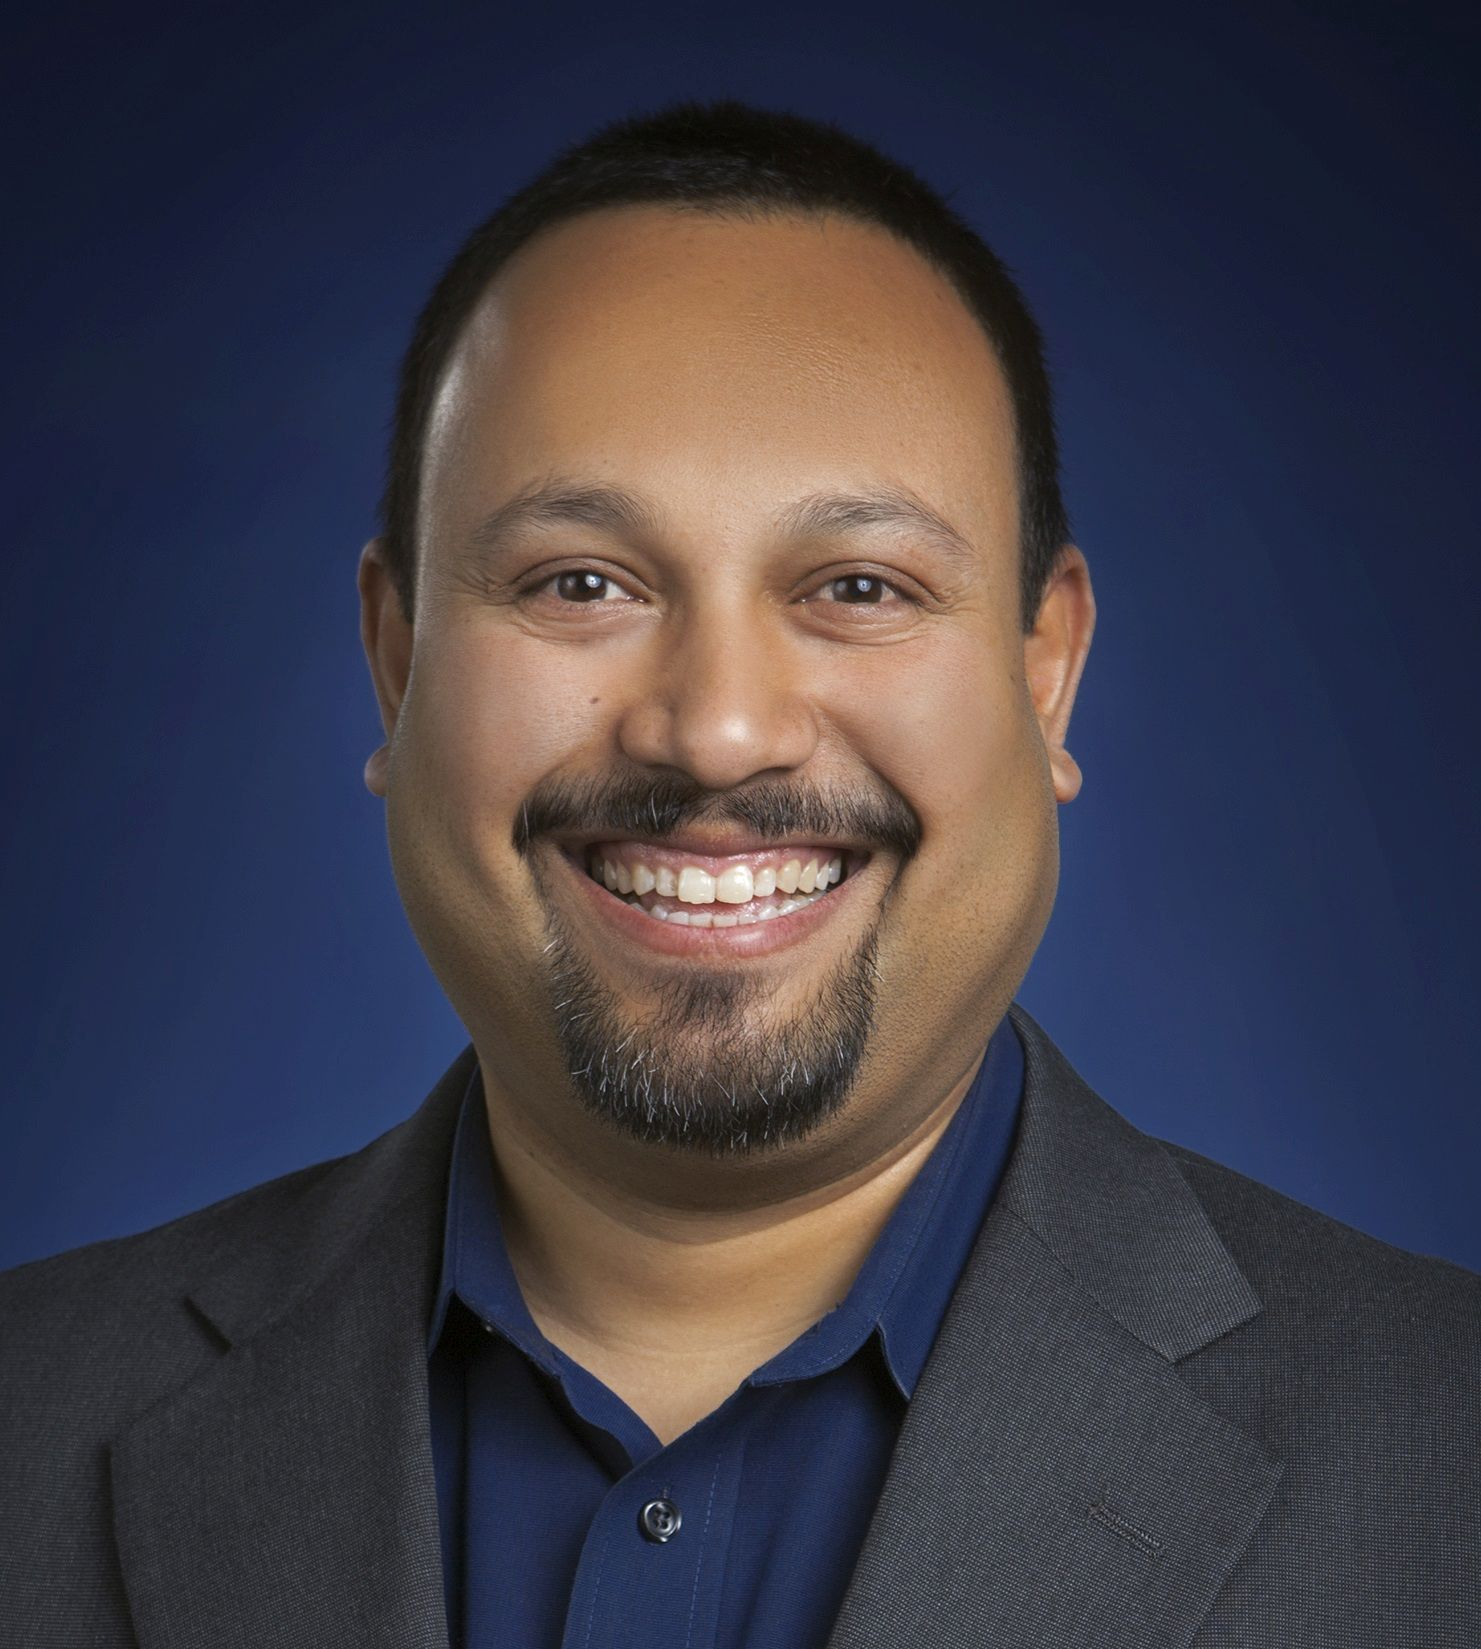
\includegraphics[width=2.60417in]{images/SanjeevKumar.jpg} \{-\}

\mainmatter

\chapter{Introduction}\label{introduction}

Welcome to \textbf{Advanced Big Data Analytics for Business with R}.
Let's get started.

\section{Archive - Delete}\label{archive---delete}

This section holds the placeholder information that will be deleted
after the book is built.

We have a nice figure in Figure \ref{fig:hello}, and also a table in
Table \ref{tab:iris}.

\begin{Shaded}
\begin{Highlighting}[]
\KeywordTok{par}\NormalTok{(}\DataTypeTok{mar =} \KeywordTok{c}\NormalTok{(}\DecValTok{4}\NormalTok{, }\DecValTok{4}\NormalTok{, }\DecValTok{1}\NormalTok{, .}\DecValTok{1}\NormalTok{))}
\KeywordTok{plot}\NormalTok{(cars, }\DataTypeTok{pch =} \DecValTok{19}\NormalTok{)}
\end{Highlighting}
\end{Shaded}

\begin{figure}
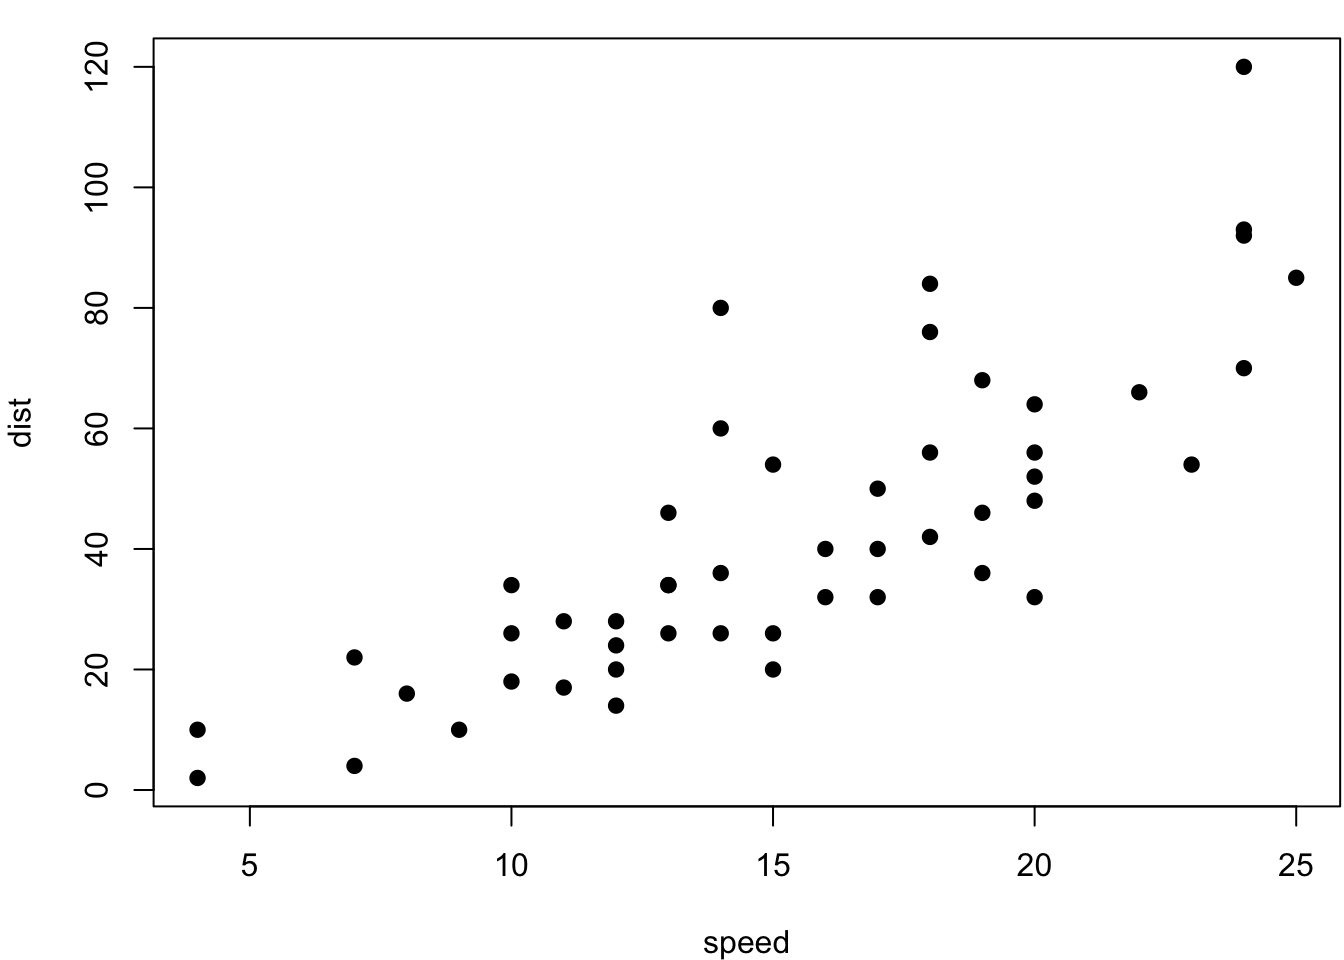
\includegraphics[width=0.9\linewidth]{bookdown_files/figure-latex/hello-1} \caption{Hello World!}\label{fig:hello}
\end{figure}

\begin{Shaded}
\begin{Highlighting}[]
\NormalTok{knitr}\OperatorTok{::}\KeywordTok{kable}\NormalTok{(}
  \KeywordTok{head}\NormalTok{(iris), }\DataTypeTok{caption =} \StringTok{'The boring iris data.'}\NormalTok{,}
  \DataTypeTok{booktabs =} \OtherTok{TRUE}
\NormalTok{)}
\end{Highlighting}
\end{Shaded}

\begin{table}

\caption{\label{tab:iris}The boring iris data.}
\centering
\begin{tabular}[t]{rrrrl}
\toprule
Sepal.Length & Sepal.Width & Petal.Length & Petal.Width & Species\\
\midrule
5.1 & 3.5 & 1.4 & 0.2 & setosa\\
4.9 & 3.0 & 1.4 & 0.2 & setosa\\
4.7 & 3.2 & 1.3 & 0.2 & setosa\\
4.6 & 3.1 & 1.5 & 0.2 & setosa\\
5.0 & 3.6 & 1.4 & 0.2 & setosa\\
5.4 & 3.9 & 1.7 & 0.4 & setosa\\
\bottomrule
\end{tabular}
\end{table}

\chapter{Advanced Big Data Analytics}\label{advanced-big-data-analytics}

Content to be added.

\chapter{Our Tools: R, RStudio}\label{our-tools-r-rstudio}

R is awesome. R is also considered pretty difficult to learn. In my
opinion, that's not true. In this chapter, we will quickly get out feet
wet in the shallow end of the R pool - ready to jump off the deep end in
the succeeding chapters.

\section{Introduction to R and
RStudio}\label{introduction-to-r-and-rstudio}

For the purpose of this course, R is a Statistical Computing
Environment. It provides us with an underlying computer language,
analysis tools and software platform for us to work with data. While R
is pretty powerful, it is built by geeks for geeks. As a result, it
lacks the user-friendliness needed by beginners and casual users. To
help mitigate this problem, we do not directly interface with R and
instead use the user friendly RStudio software as a wrapper around R.
RStudio is often considered an IDE (Integrated Development Environment)
for R.

For the record, R is a pretty awful name for anything - try googling
``R'' and see how relevant the search results are! It is called R after
the first name of the two authors of R: Robert and Ross. The name kinda
makes sense when you consider that R is based on another programming
language named S.

\subsection{Download and Install R and
RStudio}\label{download-and-install-r-and-rstudio}

R can be downloaded from any of the mirror sites maintained by the
Comprehensive R Archive Network (``CRAN''). I recommend the CRAN Mirror
maintained by RStudio: \url{https://cran.rstudio.com/}. Here you will
find links to download R for Windows, Mac-OS and Linux. The current
version of R available for Windows is R 3.4.3 and measures at around
70MB. Follow the directions to install the starting packages for R -
often called ``Base R''.

Even though we will not use a bare R installtion - lets take a look at
it anyway. Launch R once the installation finishes. It will look similar
to the figure below. This window is called the R Console. As you would
note - it looks a little scary - no icons, nothing clickable, no menu
even. While it is possible for us to do everything we wish to do with R
just with the R Console, it really would be nice to make our experience
with R a little more user friendly. Lucky for us, we have RStudio to
pick up the slack here.

\begin{figure}
\centering
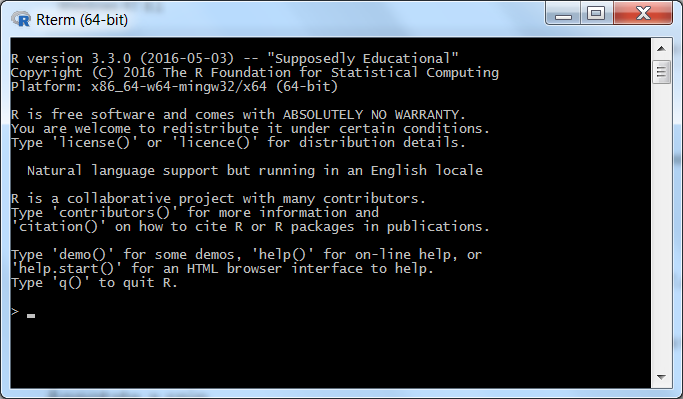
\includegraphics{images/rbase.png}
\caption{Staring Window of Base R Installation}
\end{figure}

Once you have finished installing R, you can download and install
RStudio from: \url{https://www.rstudio.com/products/rstudio/download/}.
There again are installers available for Windows, Mac-OS and Linux.
After you are done installing RStudio, you should launch RStudio to
check that everything is installed and connected properly. When you
launch RStudio for the first time, you will see something similar to the
figure below.

\begin{figure}
\centering
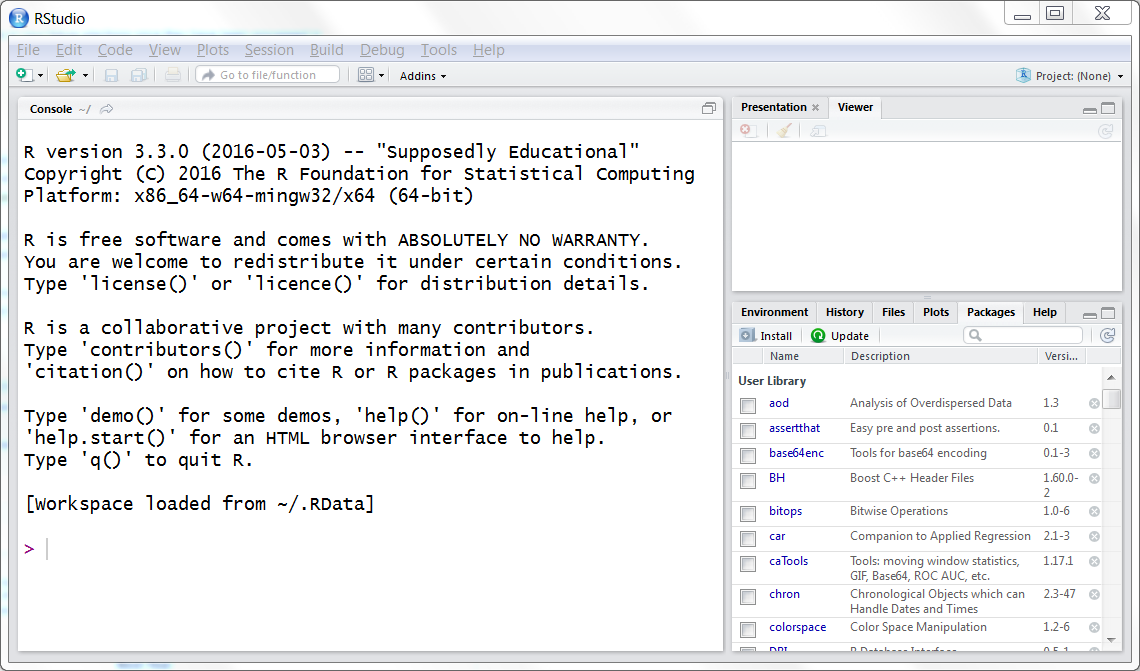
\includegraphics{images/rstudio.png}
\caption{Staring Window of RStudio}
\end{figure}

The larger part of the RStudio window is same as the R Console and this
is in-fact R running inside RStudio. When we launched R independently,
this is the prompt that you we got. RStudio combines this direct access
to R with other useful elements. In the bottom right, you have access to
the file system, you can manage R packages (more about them later), read
Help documentation and see various plots and charts that you will soon
be building. In the top right, RStudio provides you with details of
current R environment and a history of your recent R commands. If you
are using Git repository for your files then you will see Git tab here.

Now that we have both R and RStudio set up, it is time for us to get
started in making some use of it. Note that the R environment is used
primarily by typing commands on the Console prompt or running commands
saved in a file - typically a R Script file or a RMarkdown file. While
RStudio provides GUI elements for many common tasks, we will emphasize
corresponding command line versions which usually provide better control
and flexibility compared to their GUI counterparts.

\section{Useful Features of RStudio}\label{useful-features-of-rstudio}

\subsection{Console}\label{console}

The console is where you can interact directly with the R system. You
can write one line at a time and immediately execute it there by
pressing enter. If you wish to write more than one command in one line
then you can separate the commands using the semi-colon character. The
console is essentially an R session running inside RStudio. The console
shows a command prompt (usually the \texttt{\textgreater{}}\}) character
to indicate that you can type there. You can change the prompt by
changing the options setting.\footnote{I once thought it was very clever
  to have this as my prompt ``Sanjeev Says:''. I no longer think so.}

\subsection{Editor}\label{editor}

The editor is where you can work on and edit all of your files. This is
a pure text editor - so no formatting of any kind. You will mostly be
working with RMD files here. The tab panel at the top of the editor
allows you to work on multiple files at once. The editor window is
hidden when you start RStudio as you usually don't have a file to edit
when you begin. Once you create/open a new file then they will open in
the editor window and you can edit them. The editor window helpfully
shows you the line numbers in left column and the cursor positioning in
the line at the bottom left corner. The bottom right corner shows you
the file type that you are working on. There are usual icons for saving
a file, finding, spell check etc on the top bar. See Figure:
\ref{fig:editor} for an example.

\begin{figure}
\centering
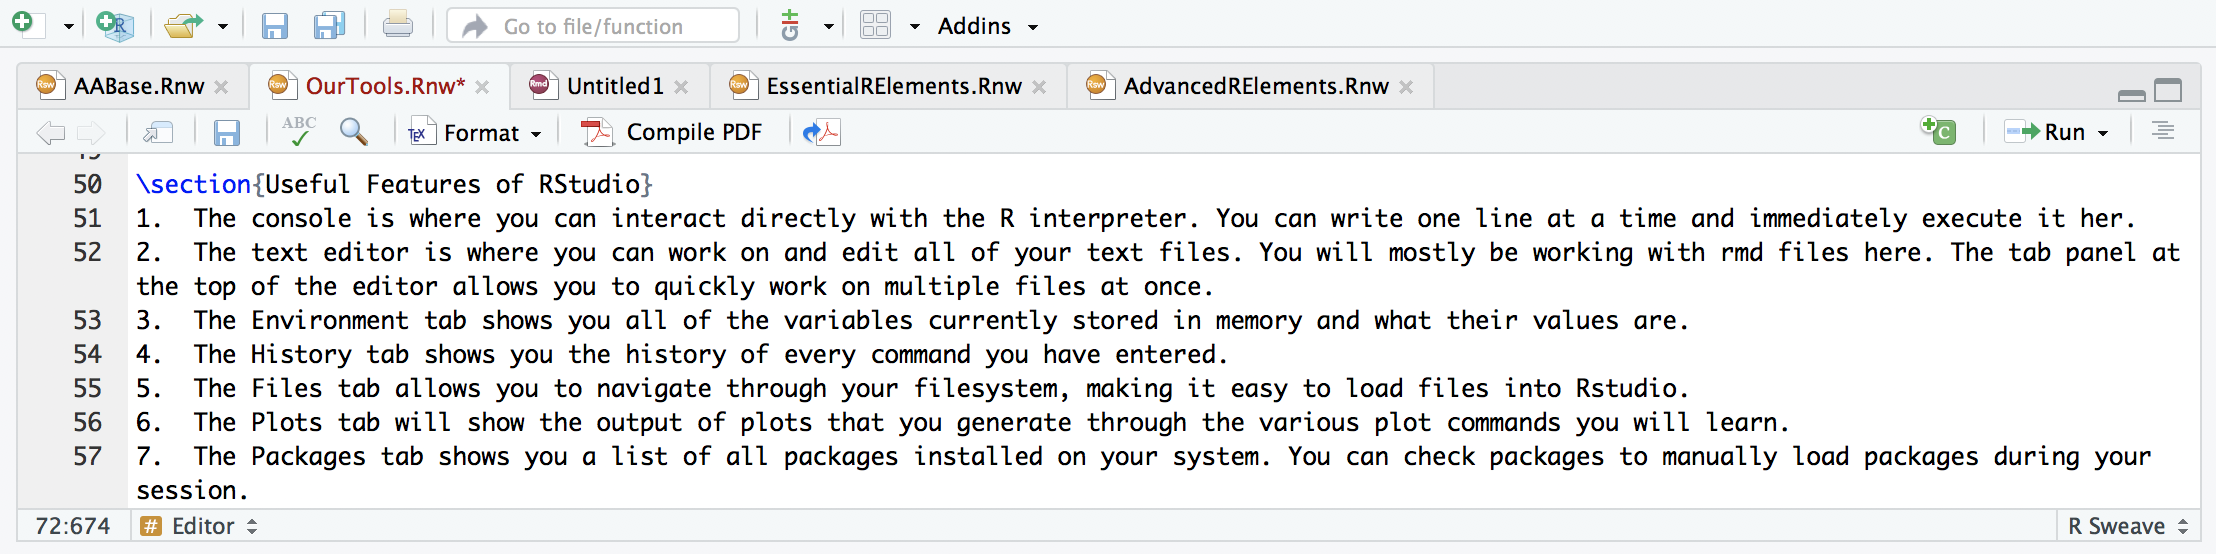
\includegraphics{images/editor.png}
\caption{RStudio Editor Window}
\end{figure}

\subsection{Environment}\label{environment}

The Environment tab shows you all of the variables currently stored in
memory and what their values are.We haven't said what variables are as
yet. Hold on - its coming in the next chapter. The tab in fact shows all
the objects that currently exist in your R session. Objects will be
discussed very soon, later in this chapter. Environment tab is a very
useful place to have a quick look at the state of your current R
session. The environment tab has a handy broom icon for deleting all the
objects that exist and clearning your environment. You can, of course,
do that using a command as well - \textbf{\texttt{rm}} for remove or
delete. The command \textbf{\texttt{ls}} generates a list of all the
objects in the environment. We can combine the two to delete every
object in the environment if we so choose:

\begin{Shaded}
\begin{Highlighting}[]
\KeywordTok{rm}\NormalTok{(}\DataTypeTok{list =} \KeywordTok{ls}\NormalTok{()) }\CommentTok{#Delete every object in the environment}
\end{Highlighting}
\end{Shaded}

\subsection{History}\label{history}

The History tab shows you the history of all the commands you have
entered in the Console window. You can use available icons on top to
search through the history or delete items from the history. Two very
useful icons are for transferring commands to the console and to the
source. See details in figure below. . The \texttt{To\ Console} option
allows you to select one or more commands from the history and transfers
them to the Console window where you can run them by pressing Enter. The
\texttt{To\ Source} option sends the selected commands to the Editor
window, to the currently open and active file.

\begin{figure}

{\centering 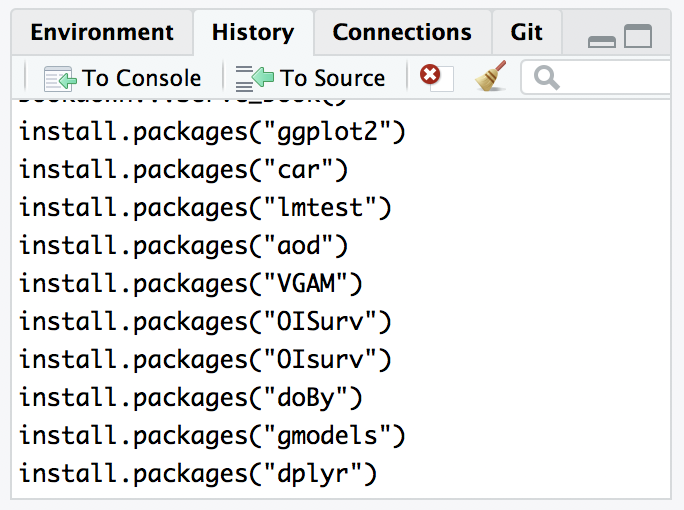
\includegraphics[width=0.5\linewidth]{images/history} 

}

\caption{RStudio History Window}\label{fig:unnamed-chunk-5}
\end{figure}

\subsection{Files}\label{files}

The Files tab allows you to navigate through your filesystem, making it
easy to load files into Rstudio. It shows the content of the current
working directory when RStudio starts. You can navigate through the file
system of your machine using the available options. The top icons
provide ability to create a new folder, delete selected files, rename
selected files and refresh file listings. The \texttt{More} option
reveals further functionalities including two useful ones: the ability
to set the currently displayed directory as the working directory and
the ability to get the Files tab to display the contents of the current
working directory. Figure: shows the options.

\begin{figure}

{\centering 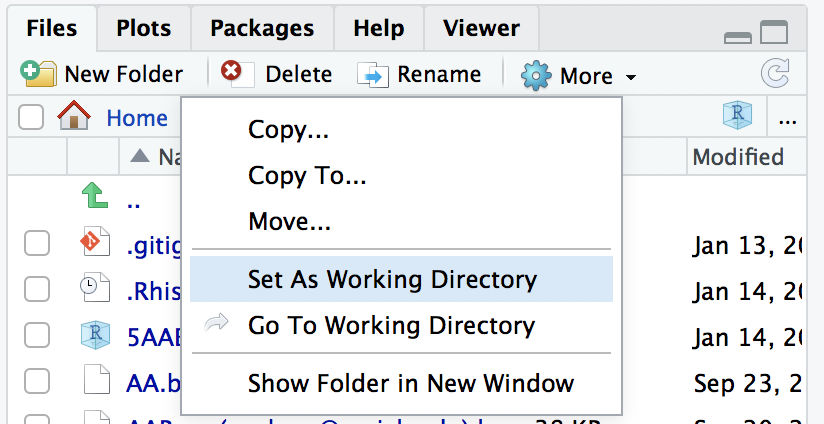
\includegraphics[width=0.5\linewidth]{images/files} 

}

\caption{RStudio Files Tab}\label{fig:unnamed-chunk-6}
\end{figure}

\subsection{Plots}\label{plots}

the Plots tab shows the plots generated by the commands typed in the
Console. See figure show the plot generated by the \texttt{plot(cars)}
command in the Plots tab. As you can see, you can use options to zoom
in/out and export the plot image as an image file or a PDF document.
Plots made by R plots are Vector graphics and hence should be saved in
vector formats like PNG and not bitmap formats like JPG.

\begin{figure}

{\centering 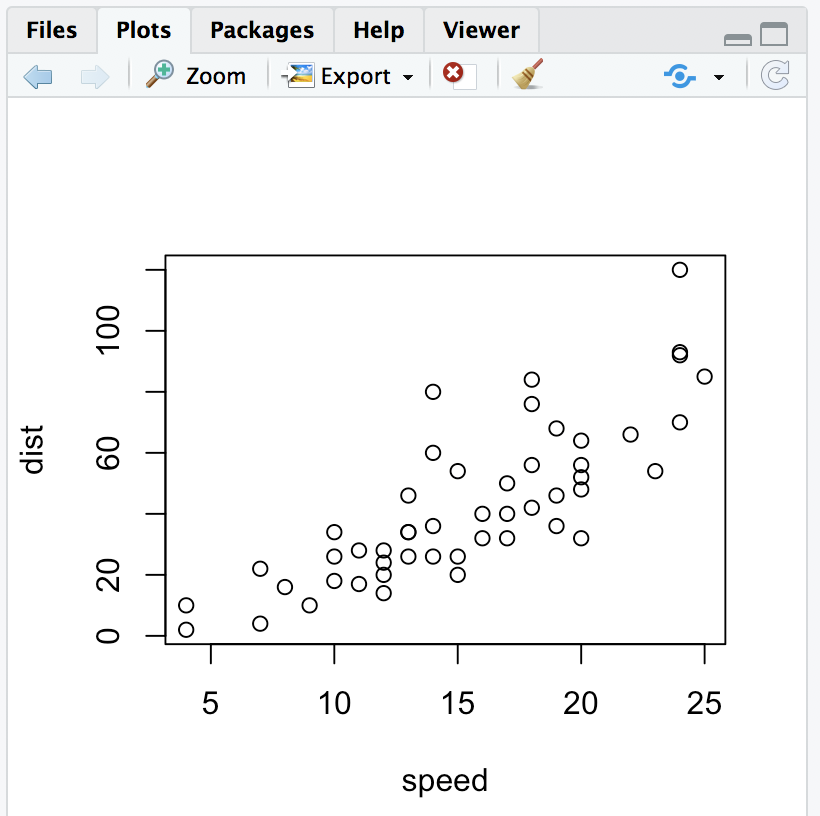
\includegraphics[width=0.5\linewidth]{images/plots} 

}

\caption{Plots Window with a Demo Plot}\label{fig:unnamed-chunk-7}
\end{figure}

\subsection{Packages}\label{packages}

The Packages tab shows you a list of all the packages installed on your
system and their version number. You can check the checkbox next to the
package name to manually load packages during your R session. You will
also find icons for installing and updating packages. A search icon
allows for searching among installed packages.

\subsection{Help}\label{help}

As the name suggests, the Help tab can be used to find Help
documentation on specific keywords. You can search for a keyword in the
search field for looking at corresponding help documentation. If you
write a help command in the console, then the output of that will also
show in the Help tab. For example, if you type the command below
(looking for help on ``help''), you will get the help documentation as
shown in figure below.

\begin{Shaded}
\begin{Highlighting}[]
\KeywordTok{help}\NormalTok{(}\StringTok{"help"}\NormalTok{)}
\end{Highlighting}
\end{Shaded}

\begin{figure}

{\centering 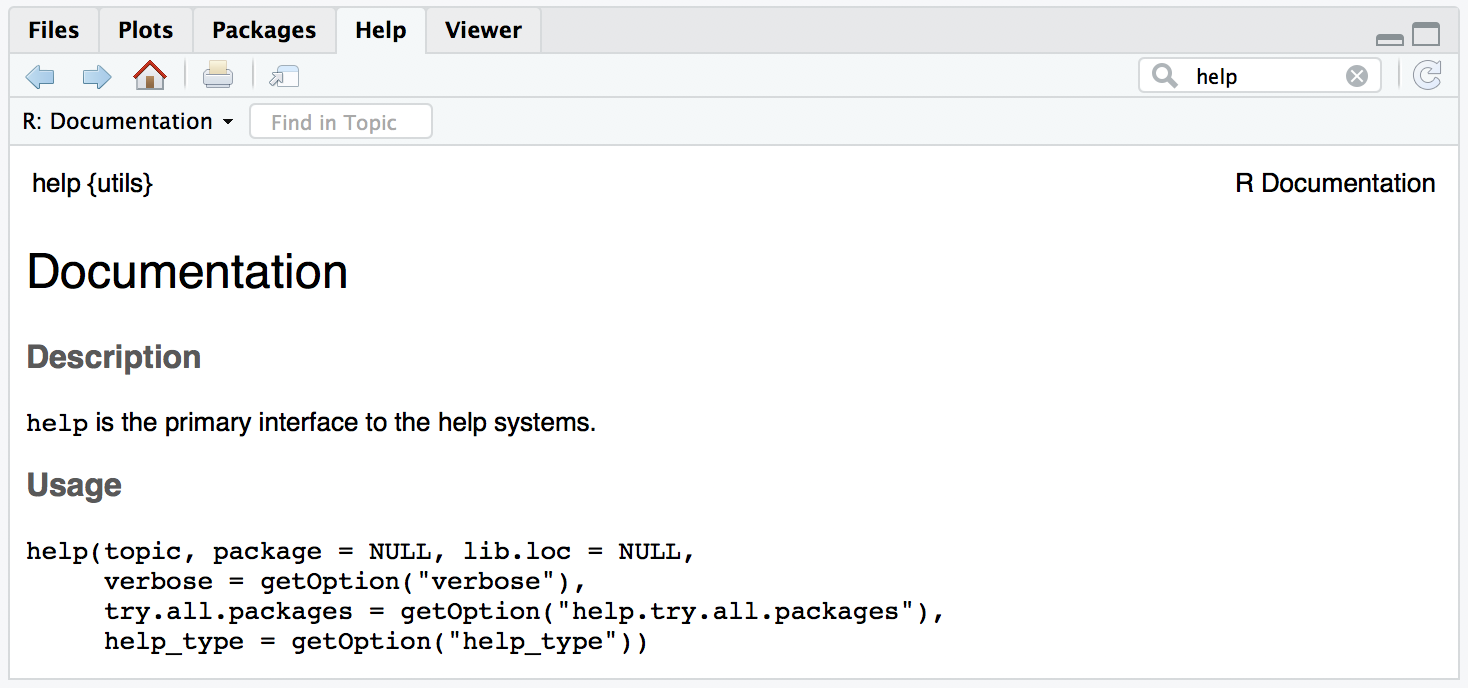
\includegraphics[width=0.8\linewidth]{images/help} 

}

\caption{Helo Window on 'Help'}\label{fig:unnamed-chunk-9}
\end{figure}

\section{Helpful Menu Items and Keyboard
Shortcuts}\label{helpful-menu-items-and-keyboard-shortcuts}

\section{Essential R Tips and Tricks}\label{essential-r-tips-and-tricks}

\subsection{R is Case Specific and Space
Neutral}\label{r-is-case-specific-and-space-neutral}

Everything in R is case specific. In R, upper case letters are
considered completely different than their lower case counterparts. R
will show no mercy if you mistype something in a difference case.
However, R is pretty flexible about spaces and will usually accept
multiple (or none) spaces where the default expectation is one space.

\subsection{Comments and Line
Continuation}\label{comments-and-line-continuation}

You can add your comments/remarks in your R code by inserting the
\texttt{\#} character. Any text after the \texttt{\#} character will be
ignored by R during execution. It is essential that sufficient comments
are added to your R code so that the code remains understandable and if
you share your code with somebody else then they have a way of figuring
out what you are trying to do, why and how.

R is smart enough to figure when the command is not finished and allows
you to continue typing on the next line. This usually works well when
there are un-finished parentheses or operators at the end. R indicates
that it is expecting further inputs by showing the character \texttt{+}
at the beginning of the next line. See figure for an example.

\begin{figure}

{\centering 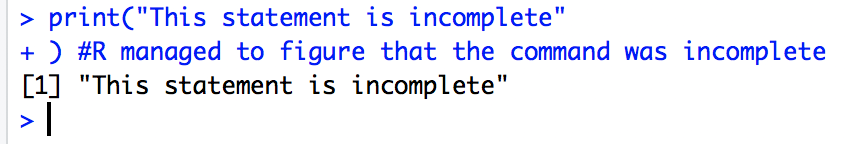
\includegraphics[width=0.5\linewidth]{images/incomplete} 

}

\caption{Line Continuation for Incomplete Commands}\label{fig:unnamed-chunk-10}
\end{figure}

\subsection{Naming Conventions}\label{naming-conventions}

Object names in R can consist of any combination of alphanumeric
characters (\texttt{a-z}, \texttt{A-Z}\}, \texttt{0-9}) as well as
underscore \texttt{-} and \texttt{.} characters. Object names should not
include special characters such as \texttt{?} or space. Object names
must start with a letter or a period. Special care should be taken to
not include one of the reserved keywords (like \texttt{function} or
\texttt{help}) as object names.

\section{RMarkdown (RMD) Files}\label{rmarkdown-rmd-files}

We will use extensive ise of RMarkdown files in the class. Markdown is a
simple formatting syntax for authoring documents. RMarkdown allows you
to create Markdown documents with embedded R code in them. RMarkdown
documents can then be rendered in variety of output formats such as
HTML, PDF, and MS Word documents.

RStudio streamlines the process of creating an RMarkdown file. Getting
started is easy - in RStudio, go File -\textgreater{} New File
-\textgreater{} R Markdown (or Alt-F-F-M). This will start a new RMD
file for you. It needs some startup information to proceed first, as
shown in the image below:

Title and Author are self explanatory. As the dialog suggests, you can
choose HTML, PDF of Word as default output formats. PDF and Word require
you to have a local installed version of TeX or MS-Word. For our class,
I recommend that you use HTML as the default output - it is device and
platform independent - and capable of handling variety of rich media. We
will see later how to include dynamic content like animation and user
interaction in these HTML files as well.

Once you say OK, you will be taken to the default start page. This page
has some content already to help you started. You should be able to see
the preamble right on top that will generate your document headers and
also control various options:

\begin{verbatim}
title: "Untitled"
author: "Dr. Sanjeev Kumar"
date: "May 5, 2018"
output: html_document
\end{verbatim}

You can make changes by either hand-editng the information above or by
clicking the Edit Option icon (which looks like a gear) and choosign
your options. For example, the preamble for one of my document looks
like the following:

\begin{verbatim}
title: "How To Write RMarkdown Files"
author: "Dr. Sanjeev Kumar"
date: "May 5, 2016"
output:
  html_document: 
    highlight: tango
    number_sections: yes
\end{verbatim}

Now you can go ahead and add content to your document. When you want to
create the output, click the \texttt{Knit} button and a document will be
generated that includes both content as well as the output of any
embedded R code chunks within the document. We will see later in the
document how to embed R code in RMD files.

It is easy to format RMarkdown files and embed R code in them. For more
details on using R Markdown see \url{http://rmarkdown.rstudio.com}.

\section{Embedding R Code Blocks in RMD
Files}\label{embedding-r-code-blocks-in-rmd-files}

\subsection{Embedding Options}\label{embedding-options}

\begin{itemize}
\tightlist
\item
  echo
\item
  eval
\item
  cache
\item
  label
\item
  fig.height/width
\end{itemize}

\subsection{Embedding Code Blocks of Other
Languages}\label{embedding-code-blocks-of-other-languages}

\subsection{Embedding in-line R Code}\label{embedding-in-line-r-code}

\subsection{Reproducibility of Data
Analysis}\label{reproducibility-of-data-analysis}

A key advantage of using an RMD file is that the output contains both
the R code and the output. That allows for a precise matching of what
steps were performed to reach a specific output. Consider the example of
a complex chart made in MS-Excel - you would be hard pressed to figure
out what exactly was done to create that chart. Whether the chart has
some data manipulation in it, whether the chart inadvertently includes a
mistake - there is no transparency - and hence you are likely to not
have much trust in the chart. In the case of RMD files on the other
hand, the entire process of creating the chart is right there in the
form of R commands. Anybody else with the same data and the same
commands will reach exactly the same output. Your analysis can be
reproduced by anybody else - imporving the reliability and
trustworthiness of your analysis.

We discussed ``veracity'' as one of the four Vs of Big Data. Doing data
analytics in a way that is reproducible (e.g through an RMD file) goes a
long way towards establishing confidence in the results of the analysis.

\section{Key Features of R/RStudio
Ecosystem}\label{key-features-of-rrstudio-ecosystem}

\subsection{Open Source Software}\label{open-source-software}

Open Source Software is a broad term for software that is developed by a
community of volunteers and is available free of charge for you and I to
use. R is open source with a strong and dedicated community that takes
the stewardship of R very very seriously.

As R is open source, the underlying computer code (the source code) is
available for anyone to view and modify. All these extra eyes looking at
the code usually means a more reliable, error free and malware resistant
software.

Open source nature of R has both positive and negative impacts. On the
positive side, the community helps extend R rapidly by building new
packages with new capabilities very quickly. On the negative side, the R
platform is built by experts for experts - the focus is on capability
and precision - not on ease of use. This makes R a swiss army knife of
that is capable of doing almost everything possible in data domain but a
knife that can be difficult to learn how to use.

\subsection{Extensability of R}\label{extensability-of-r}

R is desiged to be easily extended. You, me and everyone else can write
new functionalities for R and have it available for everyone in the
world to download and use. The R community has been writing extensions
for decades now and the result is a library of thousands of packages. If
there is anything data analysis related that you want to do, chances are
that somebody else wanted to do it too, has already built a package for
it that you can download and use.

Easy extensability of R is one of the main reasons why R remained the
most capable, cutting edge data analytical platform for decades now. R
community has written packages to allow you write SQL commands, C++
commands, build geo-maps, build predictive models - all within the R
platform. New developments tend to get incorporated in R much faster
than in competing statistical software such as Stata, SAS or SPSS.

\subsection{Usability of R}\label{usability-of-r}

R is not graphical. Much of R's capabilities are accessed through typing
R commands rather than clicking buttons or accessing menus. R commands
allow a level of precision and flexibility that is typically now
achievable through a graphical interface. Doing complex tasks
successfully in R involves writing a sequence of R commands that are
closer to coding in a programming language than using a point and click
software.

While R can be considered to have a steep learning curve, it should be
noted that once you get through the learning curve and get used to R's
syntax, you can slice through complex data analysis with much greater
speed and capability than competing alternatives. In my opinion, the
learning curves for R and competing graphical alternatives look like the
figure below. R starts slower and has a difficult jumpstart but if you
stay with it for a little bit then R handily outperforms the graphical
alternatives.

\begin{Shaded}
\begin{Highlighting}[]
\KeywordTok{curve}\NormalTok{(x}\OperatorTok{^}\DecValTok{2}\NormalTok{,}\DataTypeTok{from =} \DecValTok{0}\NormalTok{,}\DataTypeTok{to =} \DecValTok{3}\NormalTok{, }\DataTypeTok{xlab =} \StringTok{"Time"}\NormalTok{, }\DataTypeTok{ylab=}\StringTok{"Expertise"}\NormalTok{, }
      \DataTypeTok{col =} \StringTok{"red"}\NormalTok{, }\DataTypeTok{lwd=}\DecValTok{2}\NormalTok{, }\DataTypeTok{xaxt =} \StringTok{'n'}\NormalTok{, }\DataTypeTok{yaxt =} \StringTok{'n'}\NormalTok{)}
\KeywordTok{abline}\NormalTok{(}\DataTypeTok{a =} \DecValTok{2}\NormalTok{,}\DataTypeTok{b =} \DecValTok{1}\NormalTok{, }\DataTypeTok{col =} \StringTok{"blue"}\NormalTok{, }\DataTypeTok{lwd =} \DecValTok{2}\NormalTok{)}
\end{Highlighting}
\end{Shaded}

\begin{figure}
\centering
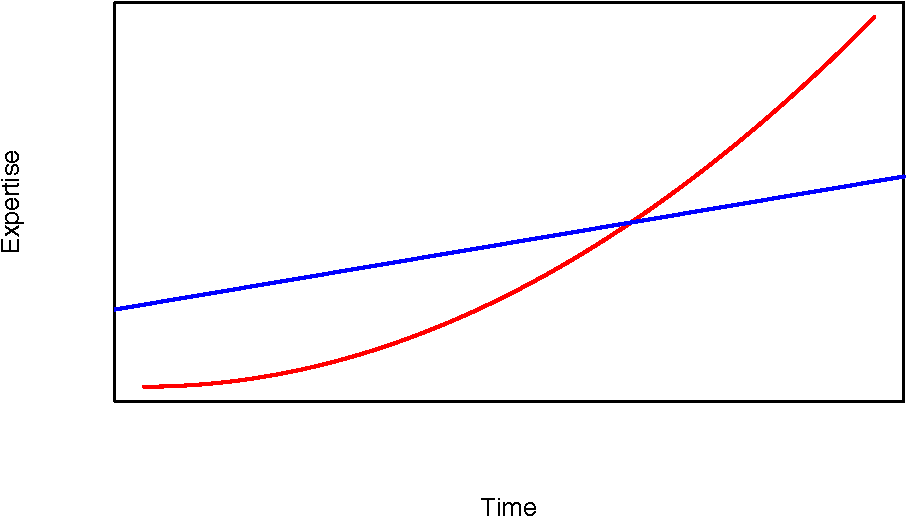
\includegraphics{bookdown_files/figure-latex/unnamed-chunk-12-1.pdf}
\caption{\label{fig:unnamed-chunk-12}Learning Curves for R (red) and
alternatives (blue)}
\end{figure}

\subsection{R is NOT Verbose}\label{r-is-not-verbose}

In fact R is very very concise. It will not give you an output until you
ask for it. This is very different than most statistical software that
tend to overwhelm the user with every possible output possible. R allows
you the flexibility to specifically request the levek of detail you
need. By default, R will provide only the minimal amount of output.

\subsection{Object Oriented
Programming}\label{object-oriented-programming}

\subsection{R Community's Sense of
Humor}\label{r-communitys-sense-of-humor}

R community is a hard working one - they are continuously building new
and latest packages - making the R ecosystem even better. R community is
also a fun one - a clever one at the very least. For example - look at
the nickname for the current version:

\begin{Shaded}
\begin{Highlighting}[]
\NormalTok{version}\OperatorTok{$}\NormalTok{nickname}
\end{Highlighting}
\end{Shaded}

\begin{verbatim}
## [1] "Kite-Eating Tree"
\end{verbatim}

The R community is very helpful and will answer your questions if you
post on relevant forums like StackExchange.com. However, they don't
suffer fools and xpect people who ask questions to have done their
homework. Over the years, the R community has developed an extensive
knowledgebase that is only a google search away for you. As you go
further in your exploration of R, attempt to learn from the community
and hopefully one day be a bonafide member of the community.

\section{Common Issues, Pitfalls, Bugs, Obstacles and Their
Solutions}\label{common-issues-pitfalls-bugs-obstacles-and-their-solutions}

This section is my master list of common issues that students encounter
when they start working with R. You may want to not read this in full
right now - treat this as a reference section. When you run into an
issue, come by here and see if I have a solution for you.

\subsection{I have an older R installtion. How do I upgrade
it?}\label{i-have-an-older-r-installtion.-how-do-i-upgrade-it}

You might have an old, not updated version of R in your machine. You can
check the current version of your R by running the \texttt{version}
command. If you have an older version and if you are in a Windows
machine, then upgrading your R installation is easy with the
\texttt{installr} package. The \texttt{installr} package has the handy
\texttt{updateR} command that will automatically update your R
installation to the latest one. A sample code to accomplish this is
below:

\begin{Shaded}
\begin{Highlighting}[]
\CommentTok{#Sample code, not being evaluated here}
\KeywordTok{install.packages}\NormalTok{(}\StringTok{"installr"}\NormalTok{) }\CommentTok{# install the installr package }
\KeywordTok{library}\NormalTok{(installr)}
\KeywordTok{updateR}\NormalTok{() }\CommentTok{# updating your R version}
\NormalTok{version }\CommentTok{# command for checking your current R version}
\end{Highlighting}
\end{Shaded}

If you happen to be in a Mac or Linux machine, then you would want to
download the current version of R and install. This process is similar
to installing a fresh new installation of R as discussion in a previous
section.

\subsection{Help - I am not being able to install any
packages!}\label{help---i-am-not-being-able-to-install-any-packages}

If you are unable to install R packages, there are a few things we can
try.\footnote{I am not going to insult your intelligence by asking you
  to make sure that you have a live Internet connection!} First thing to
check would be your anti-virus software. Several anti-virus software
balk at allowing R to perform tasks that may be interpreted as a
security risk (for example - downloading and installing packages from
the Internet). You can try to work around this by disabling/uninstalling
your anti-virus or adding R to the exceptions list in the anti-virus.

You may also want to check whether you have administrator access in the
machine you are working on. Several essential tasks in R require the
user to have administrator access.

Lastly, R may be attempting to install packages into a directory that it
does not have write permissions on. This can sometimes happen if you are
on a computer on a network with mapped drives. You can work around this
problem by asking R to install your packages in a safe, editable
directory where you have write access. R installs all packages in a
library directory - you can find out the current location of the library
directory with the \texttt{.libPaths} command. You can use the
\texttt{.libPaths} command to then add a directory location as your
personal library location so that R can then install packages in that
directory. A sample code to accomplish this is shown below: \footnote{Last
  command commented as C:/Whatever does not exist obviously - so would
  have resulted in an error - hence it is commented out.}

\begin{Shaded}
\begin{Highlighting}[]
\KeywordTok{.libPaths}\NormalTok{() }\CommentTok{#Shows the current library path}
\end{Highlighting}
\end{Shaded}

\begin{verbatim}
## [1] "/Library/Frameworks/R.framework/Versions/3.4/Resources/library"
\end{verbatim}

\begin{Shaded}
\begin{Highlighting}[]
\CommentTok{# You can add your own library folder to the path}
\CommentTok{#libPaths( c( .libPaths(), "C:/Whatever/Whatever...") )}
\end{Highlighting}
\end{Shaded}

\subsection{Why is the edit command not working for
me?}\label{why-is-the-edit-command-not-working-for-me}

One of the first R commands that gives trouble is the \texttt{edit}
command. As the name suggests, \texttt{edit} is used for editing data -
typically it shows the data to be edited in a table format with editable
cells. This specific command (and its cousin, the \texttt{fix} command)
seems to be very sensitive to the keyboard layouts, especially on Apple
machines. This problem is hardware oriented and may prove difficult to
solve. I usually recommend to ignore these two commands and take care of
your data editing needs using alternative methods. If you were using
\texttt{edit} for only viewing the data, then \texttt{View} is a good
alternative for that.

\chapter{Essential R Language
Elements}\label{essential-r-language-elements}

In this chapter we will start playing with some basic R functionalities
and start getting comfortable with typing commands in the R console. All
code examples you see in the chapter are opportunities for you to type
them in R Console yourself and see whether you get the same output.
There is no better way to find your way around R than to get your hands
dirty - and no better time than now. So lets get started.

\section{Doing Calculations - Arithmatic
Operators}\label{doing-calculations---arithmatic-operators}

You can use R as a glorified calculator. All arithmatic calculations can
be easily performed using Arithmatic Operators like \texttt{+}
(addition), \texttt{-} (subtraction), \texttt{*} (multiplication),
\texttt{/} (division) and \texttt{\^{}} (exponent).

\begin{Shaded}
\begin{Highlighting}[]
\DecValTok{10}  \OperatorTok{+}\StringTok{    }\DecValTok{20}  \CommentTok{#As you can see - spaces don't matter, mostly.}
\end{Highlighting}
\end{Shaded}

\begin{verbatim}
## [1] 30
\end{verbatim}

\begin{Shaded}
\begin{Highlighting}[]
\DecValTok{20}\OperatorTok{/}\DecValTok{3} \CommentTok{#Note the nunber of digits after decimal}
\end{Highlighting}
\end{Shaded}

\begin{verbatim}
## [1] 6.667
\end{verbatim}

\begin{Shaded}
\begin{Highlighting}[]
\DecValTok{16} \OperatorTok{^}\StringTok{ }\FloatTok{0.5}  \CommentTok{# Usual Arithmatic Operators: +, -, * , /, ^}
\end{Highlighting}
\end{Shaded}

\begin{verbatim}
## [1] 4
\end{verbatim}

You would note that the outputs to the commands have this
\texttt{{[}1{]}} before them. The number indicates how many values there
are in the output. Since each of the commands above lead to a single
output value - you see the \texttt{{[}1{]}} there before the output.

When you have complicated Arithmatic Expressions, R follows usual
Arithmatic Operator Precedance: Brackets, Exponent, Division and
Multiplication, Addition and Subtraction - in that order. Go Left to
Right for the same precedance. Of course it is preferable to put in
enough paratheses so that you are not relying on R's operator precedance
for accurate execution of your commands.

\begin{Shaded}
\begin{Highlighting}[]
\DecValTok{5} \OperatorTok{+}\StringTok{ }\DecValTok{8} \OperatorTok{/}\StringTok{ }\DecValTok{2} \OperatorTok{*}\StringTok{ }\DecValTok{4} \OperatorTok{-}\StringTok{ }\DecValTok{3} \CommentTok{# First * then / then + then - }
\end{Highlighting}
\end{Shaded}

\begin{verbatim}
## [1] 18
\end{verbatim}

\begin{Shaded}
\begin{Highlighting}[]
\CommentTok{# You should include enough parantheses}
\NormalTok{(}\DecValTok{5} \OperatorTok{+}\StringTok{ }\DecValTok{8}\NormalTok{) }\OperatorTok{/}\NormalTok{((}\DecValTok{2} \OperatorTok{*}\StringTok{ }\DecValTok{4}\NormalTok{) }\OperatorTok{-}\StringTok{ }\DecValTok{3}\NormalTok{)}
\end{Highlighting}
\end{Shaded}

\begin{verbatim}
## [1] 2.6
\end{verbatim}

Two arithmatic operators that many are not familiar with are: Integer
Division and Remainder operators. The Integer Division operator:
\texttt{\%/\%}, provides just the quotient for a division operation
while the remainder operator: \texttt{\%\%}, provides just the remainder
for a division operation.

\begin{Shaded}
\begin{Highlighting}[]
\DecValTok{10} \OperatorTok\StringTok{ }\DecValTok{3} \CommentTok{# Integer division - only gives the quotient as the output}
\end{Highlighting}
\end{Shaded}

\begin{verbatim}
## [1] 3
\end{verbatim}

\begin{Shaded}
\begin{Highlighting}[]
\DecValTok{10} \OperatorTok\StringTok{ }\DecValTok{3} \CommentTok{# The counterpart to %/%, gives remainder as the output}
\end{Highlighting}
\end{Shaded}

\begin{verbatim}
## [1] 1
\end{verbatim}

\section{Logical Operators}\label{logical-operators}

Just as arithmatic expressions evaluate to a numerical result, logical
expressions evaluate to a logical result - either \texttt{TRUE} or
\texttt{FALSE}. Note the upper case format for the two keywords. The
letters \texttt{T} and \texttt{F} are also acceptable values as
shorthand for \texttt{TRUE} and \texttt{FALSE}. Logical expressions can
be created using Logical Operators: equal to (\texttt{==}), greate than
(\texttt{\textgreater{}}), less than (\texttt{\textless{}}), greater
than or equal to (\texttt{\textgreater{}=}), less than or equal to
(\texttt{\textless{}=}) and finally, not equal to (\texttt{!=}).

\begin{Shaded}
\begin{Highlighting}[]
\DecValTok{10} \OperatorTok{>}\StringTok{ }\DecValTok{20} \CommentTok{#Should evaluate to FALSE}
\end{Highlighting}
\end{Shaded}

\begin{verbatim}
## [1] FALSE
\end{verbatim}

\begin{Shaded}
\begin{Highlighting}[]
\FloatTok{12.37} \OperatorTok{<=}\StringTok{ }\FloatTok{23.66} \CommentTok{#Should evaluate to TRUE}
\end{Highlighting}
\end{Shaded}

\begin{verbatim}
## [1] TRUE
\end{verbatim}

\begin{Shaded}
\begin{Highlighting}[]
\NormalTok{(}\DecValTok{10}\OperatorTok{/}\DecValTok{3}\NormalTok{) }\OperatorTok{==}\StringTok{ }\NormalTok{(}\DecValTok{30}\OperatorTok{/}\DecValTok{9}\NormalTok{) }\CommentTok{#Should evaluate to TRUE}
\end{Highlighting}
\end{Shaded}

\begin{verbatim}
## [1] TRUE
\end{verbatim}

Logical values can be combined using \texttt{AND} and \texttt{OR}
constructs. When combining two logical values using \texttt{OR}, the
resulting value is \texttt{TRUE} if any of the two values are
\texttt{TRUE}. When combining two logical values using \texttt{AND}, the
resulting value is \texttt{TRUE} only of both the values are
\texttt{TRUE}. The command for \texttt{AND} is \texttt{\&} while the
command for \texttt{OR} is the \texttt{\textbar{}} character.

\begin{Shaded}
\begin{Highlighting}[]
\NormalTok{(}\DecValTok{10} \OperatorTok{>}\StringTok{ }\DecValTok{20}\NormalTok{) }\OperatorTok{|}\StringTok{ }\NormalTok{(}\FloatTok{12.37} \OperatorTok{<=}\StringTok{ }\FloatTok{23.66}\NormalTok{) }\CommentTok{#Should evaluate to TRUE}
\end{Highlighting}
\end{Shaded}

\begin{verbatim}
## [1] TRUE
\end{verbatim}

\begin{Shaded}
\begin{Highlighting}[]
\NormalTok{(}\DecValTok{10} \OperatorTok{>}\StringTok{ }\DecValTok{20}\NormalTok{) }\OperatorTok{&}\StringTok{ }\NormalTok{(}\FloatTok{12.37} \OperatorTok{<=}\StringTok{ }\FloatTok{23.66}\NormalTok{) }\CommentTok{#Should evaluate to FALSE}
\end{Highlighting}
\end{Shaded}

\begin{verbatim}
## [1] FALSE
\end{verbatim}

You can use the \texttt{NOT} operator to convert a \texttt{TRUE} value
to \texttt{FALSE} and vice versa - the corresponding command is the
\texttt{!} character. You can use logical operators to compare
non-numeric values as well.

\begin{Shaded}
\begin{Highlighting}[]
\OperatorTok{!}\OtherTok{TRUE} \CommentTok{#Should evaluate to FALSE}
\end{Highlighting}
\end{Shaded}

\begin{verbatim}
## [1] FALSE
\end{verbatim}

\begin{Shaded}
\begin{Highlighting}[]
\StringTok{"Dog"} \OperatorTok{>}\StringTok{ "Cat"} \CommentTok{#As everybody know, this is TRUE}
\end{Highlighting}
\end{Shaded}

\begin{verbatim}
## [1] TRUE
\end{verbatim}

As the example above shows, comparing non-numeric values can result in
interesting results \footnote{We have not discussed different data types
  yet. Values enclosed in quote marks are text values, typically called
  Strings}. When two strings are compared, they are essentially compared
one character at a time. In the example above, the character C is
compared with character D. The comparison is based on the Unicode number
associated with the characters. As D has a higher Unicode number than C,
``Dog'' is considered higher than ``Cat''. Interesting thought
experiment: 1000 \textgreater{} 50: True or False? ``1000''
\textgreater{} ``50'': True or False?

\begin{Shaded}
\begin{Highlighting}[]
\DecValTok{1000} \OperatorTok{>}\StringTok{ }\DecValTok{50}
\end{Highlighting}
\end{Shaded}

\begin{verbatim}
## [1] TRUE
\end{verbatim}

\begin{Shaded}
\begin{Highlighting}[]
\StringTok{"1000"} \OperatorTok{>}\StringTok{ "50"}
\end{Highlighting}
\end{Shaded}

\begin{verbatim}
## [1] FALSE
\end{verbatim}

\section{Variables}\label{variables}

R keeps all data in \textbf{Variables}. Variables can be thought of as a
space in computer's memory where R can store data. Once we have created
a variable, we can then use the variable name to access, manipulate and
work with the data kept in the variable. Variables are created using the
\textbf{Assignment Operator} written as \texttt{\textless{}-}. The arrow
indicates the direction of assignment. Operators also exist to do
assignment in the opposite direction \texttt{-\textgreater{}} and do the
same operation as assignment operator. R also supports the assignment
operator command used by many other programming languages \texttt{=},
but it is customary to use the right-to-left version of assignment
operator. \footnote{I find the R version of assignment operator to be
  much more intuitive as the direction of value assignment is clearly
  specified. The \texttt{=} charater usually confuses beginners into
  thinking that we are ``equating'' values instead of the correct
  interpretation of ``assigning'' value from one side to the other.}

\begin{Shaded}
\begin{Highlighting}[]
\NormalTok{revenue <-}\StringTok{ }\DecValTok{100} \CommentTok{#Typical way of creating a variable and assigning value}
\CommentTok{# Above is the recommended approach}
\NormalTok{revenue =}\StringTok{ }\DecValTok{100} \CommentTok{#Alternate way of doing same as above}
\CommentTok{#100 -> revenue #Reverse direction assignment}
\NormalTok{revenue <-}\StringTok{ }\NormalTok{revenue }\OperatorTok{+}\StringTok{ }\DecValTok{300} \CommentTok{#Performing calculations}
\KeywordTok{print}\NormalTok{(revenue) }\CommentTok{#Printing/showing the value inside the variable}
\end{Highlighting}
\end{Shaded}

\begin{verbatim}
## [1] 400
\end{verbatim}

The first three line of the code above should be read as the value 100
is assigned to the variable \texttt{revenue}. In the fourth line, we add
300 to the current value of variable \texttt{revenue} and the resulting
value (in this case 400) is then assigned to the variable
\texttt{revenue}. So the value in the variable \texttt{revenue} is now
400, which is shown as output in the last line.

A numeric variable like \texttt{revenue} above can be used just like a
number to perform all usual arithmetic operations.

\section{Variable Data Types}\label{variable-data-types}

Variables can store different types of data. We saw integer numerical
data in the examples above. Other common data types include floating
point numbers (fractional numbers), characters data (i.e.~a single
character), text data (called strings - as in string of characters) and
logical data (true or false). We can find the data type of a variable by
using the \texttt{class} command.

\begin{Shaded}
\begin{Highlighting}[]
\NormalTok{numvalue <-}\StringTok{ }\FloatTok{20.56} \CommentTok{#Creating a numeric variable}
\KeywordTok{class}\NormalTok{(numvalue) }\CommentTok{#Finding data type of numvalue variable}
\end{Highlighting}
\end{Shaded}

\begin{verbatim}
## [1] "numeric"
\end{verbatim}

\subsection{Numeric Data}\label{numeric-data}

Variables of numeric data type can store both integers and floating
point values. Unlike many programming languages, R does not have various
different kinds of integers and floating point numbers defined to
optimize memory usage.

\subsection{String Data}\label{string-data}

\textbf{String} or text data \footnote{Text is nothing but a string of
  characters, hence the name String} is written within quote marks
\texttt{"\ "} to differentiate them from text that represent things like
object names. An empty string (a text data with no characters) is
usually represented by two quote marks with nothing within - like
\texttt{""}.

\begin{Shaded}
\begin{Highlighting}[]
\NormalTok{day.name <-}\StringTok{ "Sunday"} \CommentTok{#Assigns the string Sunday to variable day.name}
\NormalTok{someday <-}\StringTok{ ""} \CommentTok{#Empty string assigned to variable someday}
\end{Highlighting}
\end{Shaded}

String is a very useful data type as all other types of data can be
saved as a string. For example - we can save numeric data (``23.37''),
date data (``12/27/1976''), logical data (``TRUE'') etc. all as string.
R has several useful commands for working with string data. You can
connect two strings together using the \textbf{String Concatenation}
function \textbf{\texttt{paste}}. You can calculate the number of
characters in a string using the \textbf{\texttt{nchar}} function. Many
other strings related commands are discussed later in this book.

\begin{Shaded}
\begin{Highlighting}[]
\KeywordTok{nchar}\NormalTok{(day.name); }\KeywordTok{nchar}\NormalTok{(someday)}
\end{Highlighting}
\end{Shaded}

\begin{verbatim}
## [1] 6
\end{verbatim}

\begin{verbatim}
## [1] 0
\end{verbatim}

\begin{Shaded}
\begin{Highlighting}[]
\NormalTok{message <-}\StringTok{ }\KeywordTok{paste}\NormalTok{(day.name, }\StringTok{" is a great day!"}\NormalTok{); message}
\end{Highlighting}
\end{Shaded}

\begin{verbatim}
## [1] "Sunday  is a great day!"
\end{verbatim}

\section{Logical Data}\label{logical-data}

Variables can hold logical values using the two keywords \texttt{TRUE}
and \texttt{FALSE}. Logical values typically result from the use of
logical operators such as the equality operator \texttt{==}. Note the
two \texttt{=} signs there which differetiates it from the version of
assignment operator we saw before.

\begin{Shaded}
\begin{Highlighting}[]
\DecValTok{4} \OperatorTok{==}\StringTok{ }\DecValTok{6} \CommentTok{#Is 4 equal to 6, result FALSE}
\end{Highlighting}
\end{Shaded}

\begin{verbatim}
## [1] FALSE
\end{verbatim}

\begin{Shaded}
\begin{Highlighting}[]
\NormalTok{someday }\OperatorTok{==}\StringTok{ "Tuesday"} \CommentTok{#Again result shoukd be FALSE}
\end{Highlighting}
\end{Shaded}

\begin{verbatim}
## [1] FALSE
\end{verbatim}

\section{Converting Between Data
Types}\label{converting-between-data-types}

Its easy to convert variables from one data type to another. Conversion
functions usually take the form of \textbf{\texttt{as.xxx}} where
\texttt{xxx} is the desired datatype. For example: \texttt{as.string}
converts to a String, \texttt{as.numeric} converts to a numeric data
type and so on.

\begin{Shaded}
\begin{Highlighting}[]
\NormalTok{x <-}\StringTok{ "12.36"} \CommentTok{#Creating a String variable}
\NormalTok{y <-}\StringTok{ }\KeywordTok{as.numeric}\NormalTok{(x); y }\CommentTok{#Converting to a numeric value and displaying}
\end{Highlighting}
\end{Shaded}

\begin{verbatim}
## [1] 12.36
\end{verbatim}

\section{Vectors}\label{vectors}

Variables store a single value. If you need to store multiple values
then you need a \textbf{\texttt{Vector}}. Vectors can be created in the
same way a variables are created, except that we can assign multiple
values to a vector. A handy function for combining multiple values in
one vector is the \textbf{combine} function written as \texttt{c}.

\begin{Shaded}
\begin{Highlighting}[]
\NormalTok{grades <-}\StringTok{ }\KeywordTok{c}\NormalTok{(}\FloatTok{3.2}\NormalTok{, }\DecValTok{3}\NormalTok{,}\DecValTok{1}\NormalTok{, }\FloatTok{2.7}\NormalTok{, }\FloatTok{3.9}\NormalTok{, }\FloatTok{4.0}\NormalTok{) }\CommentTok{#Grades of five students}
\KeywordTok{class}\NormalTok{(grades) }\CommentTok{#A vector with numeric values}
\end{Highlighting}
\end{Shaded}

\begin{verbatim}
## [1] "numeric"
\end{verbatim}

The code above created a vector named \texttt{grades} that has 5
elements. Vectors are very useful because R provides several easy ways
to interact with different elements of a vector. We can access
individual elements of a vector using the \texttt{{[}\ {]}} notation -
called \textbf{Logical Indexing}. We can use the
\textbf{\texttt{length}} function to find out how many elements there
are in the vector.

\begin{Shaded}
\begin{Highlighting}[]
\NormalTok{grades[}\DecValTok{2}\NormalTok{] }\CommentTok{#Gets the second element of the vector}
\end{Highlighting}
\end{Shaded}

\begin{verbatim}
## [1] 3
\end{verbatim}

\begin{Shaded}
\begin{Highlighting}[]
\NormalTok{grades[}\DecValTok{4}\NormalTok{] <-}\StringTok{ }\DecValTok{3} \CommentTok{#Changes 4th element of the vector to 3}
\KeywordTok{length}\NormalTok{(grades) }\CommentTok{#Gets the length (number of elements) of the vector}
\end{Highlighting}
\end{Shaded}

\begin{verbatim}
## [1] 6
\end{verbatim}

\begin{Shaded}
\begin{Highlighting}[]
\NormalTok{grades }\OperatorTok{-}\StringTok{ }\FloatTok{0.1} \CommentTok{#Adds 2 to *each* element of the vector }
\end{Highlighting}
\end{Shaded}

\begin{verbatim}
## [1] 3.1 2.9 0.9 2.9 3.8 3.9
\end{verbatim}

\begin{Shaded}
\begin{Highlighting}[]
\NormalTok{grades }\CommentTok{#Displays current elements of the vector}
\end{Highlighting}
\end{Shaded}

\begin{verbatim}
## [1] 3.2 3.0 1.0 3.0 3.9 4.0
\end{verbatim}

Vectors are also useful for doing element-by-element calculations. For
example, if we have another vector for number of hours of work for the
week, we can calculate number of hours used for work and sleep as
follows:

\begin{Shaded}
\begin{Highlighting}[]
\NormalTok{work.per.day <-}\StringTok{ }\KeywordTok{c}\NormalTok{(}\DecValTok{9}\NormalTok{, }\DecValTok{11}\NormalTok{, }\DecValTok{10}\NormalTok{, }\DecValTok{8}\NormalTok{, }\DecValTok{6}\NormalTok{, }\DecValTok{3}\NormalTok{, }\DecValTok{2}\NormalTok{) }\CommentTok{#Create new vector}
\NormalTok{sleep.per.day <-}\StringTok{ }\KeywordTok{c}\NormalTok{(}\DecValTok{6}\NormalTok{, }\DecValTok{7}\NormalTok{, }\DecValTok{4}\NormalTok{, }\DecValTok{10}\NormalTok{, }\DecValTok{8}\NormalTok{, }\DecValTok{7}\NormalTok{, }\DecValTok{11}\NormalTok{)}
\NormalTok{work.and.sleep <-}\StringTok{ }\NormalTok{sleep.per.day }\OperatorTok{+}\StringTok{ }\NormalTok{work.per.day }
\CommentTok{#Added two vectors element by element}
\KeywordTok{print}\NormalTok{(work.and.sleep) }\CommentTok{#Show added values}
\end{Highlighting}
\end{Shaded}

\begin{verbatim}
## [1] 15 18 14 18 14 10 13
\end{verbatim}

It is easy to access data elements inside a vector. All elements are
assigned an index number - unlike many programming languages, R starts
counting with 1 rather than 0.

\begin{Shaded}
\begin{Highlighting}[]
\NormalTok{wed.hours <-}\StringTok{ }\NormalTok{work.per.day[}\DecValTok{3}\NormalTok{] }\CommentTok{#Extracts third element}
\NormalTok{work.per.day[}\DecValTok{7}\NormalTok{] <-}\StringTok{ }\DecValTok{6} \CommentTok{#Changes 7th element of the vector}
\end{Highlighting}
\end{Shaded}

Functions \texttt{edit} and \texttt{fix} can be used to edit existing
vectors. Number of elements in a vector can be calculated using the
\texttt{length} function.

\begin{Shaded}
\begin{Highlighting}[]
\KeywordTok{length}\NormalTok{(work.per.day)}
\end{Highlighting}
\end{Shaded}

\begin{verbatim}
## [1] 7
\end{verbatim}

\section{Factors}\label{factors}

\section{Using Built-In Functions}\label{using-built-in-functions}

R includes many \textbf{functions\emph{\}\textbf{. Functions take some
values as inputs (often called }arguments\textbf{), perform some
calculation and return the result. For example \texttt{sqrt()}, the
}square root function}\}} takes a value and returns its square root.

\begin{Shaded}
\begin{Highlighting}[]
\KeywordTok{sqrt}\NormalTok{(}\DecValTok{100}\NormalTok{) }\CommentTok{#Calculate square root of 100}
\end{Highlighting}
\end{Shaded}

\begin{verbatim}
## [1] 10
\end{verbatim}

R includes perhaps thousands of functions for different tasks. Some
functions can take several arguments with many of them being optional.
Such optional arguments typically have a default value that is used in
case a value is not provided for that argument. When supplying several
arguments, it is a good practice to used **named arguments*\}** as shown
below.

\begin{Shaded}
\begin{Highlighting}[]
\CommentTok{#Calling functions with name arguments}
\KeywordTok{round}\NormalTok{(}\DataTypeTok{x =} \FloatTok{1.23456789}\NormalTok{, }\DataTypeTok{digits =} \DecValTok{4}\NormalTok{) }
\end{Highlighting}
\end{Shaded}

\begin{verbatim}
## [1] 1.235
\end{verbatim}

\begin{Shaded}
\begin{Highlighting}[]
\CommentTok{#Arguments passed in order, withour names}
\KeywordTok{round}\NormalTok{(}\FloatTok{1.23456789}\NormalTok{, }\DecValTok{4}\NormalTok{)}
\end{Highlighting}
\end{Shaded}

\begin{verbatim}
## [1] 1.235
\end{verbatim}

\begin{Shaded}
\begin{Highlighting}[]
\CommentTok{#Using default values for optional arguments}
\KeywordTok{round}\NormalTok{(}\FloatTok{1.23456789}\NormalTok{) }
\end{Highlighting}
\end{Shaded}

\begin{verbatim}
## [1] 1
\end{verbatim}

The first line above shows running (or calling) the function
\texttt{round} with explicitly named arguments. \texttt{x} represents
the number to be rounded and \texttt{digits} represents how many digits
after the decimal point should the rounding be done for. We could have
called the function without named arguments (like in the second line
above) but then we would need to provide all the arguments in the exact
order needed. As it is easy to mix-up the order, it is recommended that
named arguments are used when multiple arguments are passed to a
function.

The third line in the code above shows what happens when an optional
argument is not provided to a function. As we have not specified the
number of digits, the function uses the default value of the argument
(which happens to be \texttt{0} in this case). As a result, the
functions rounds the number to an integer.

Your R is only as good as your R Packages - so lets figure that first
how to install a package - you can do through RStudio GUI - or use the
command below. Note the quote marks around the package name - which,
like most other things in R, are case sensitive.

\begin{Shaded}
\begin{Highlighting}[]
\KeywordTok{install.packages}\NormalTok{(}\StringTok{"ggplot2"}\NormalTok{)}
\end{Highlighting}
\end{Shaded}

Installing is only the first step - that brings the package to your
local machine but does not load it into the current R session. To do so,
you can use the \textbf{\texttt{library}} command. You can use the
\textbf{\texttt{detach}} commans to unload a package from the current R
session. There are several thousand packages in R - waiting for us to
explore

\begin{Shaded}
\begin{Highlighting}[]
\KeywordTok{library}\NormalTok{(ggplot2)}
\KeywordTok{detach}\NormalTok{(package}\OperatorTok{:}\NormalTok{ggplot2)}
\end{Highlighting}
\end{Shaded}

You typically work in a directory during a R session. You can find
current working directory or set working directory to a directory of
your choice. When setting working directory to the desired location, in
Windows use \texttt{/} or \texttt{\textbackslash{}\textbackslash{}}
instead of \texttt{\textbackslash{}} character as the separator
character.

\begin{Shaded}
\begin{Highlighting}[]
\KeywordTok{getwd}\NormalTok{()}
\end{Highlighting}
\end{Shaded}

\begin{verbatim}
## [1] "/Users/sankum/Box Sync/2Teaching/AABookDown"
\end{verbatim}

\begin{Shaded}
\begin{Highlighting}[]
\CommentTok{#setwd("Enter Directory Addess Here")}
\end{Highlighting}
\end{Shaded}

You usually have a *\textbf{home directory} defined for your R
installation. When you start R, your R session will usually start in
this home directory. Home directory is usually referred using the
\texttt{\textasciitilde{}} character. You can find out the directory
assigned the \textbf{Home} status using the command
\texttt{path.expand}.

\begin{Shaded}
\begin{Highlighting}[]
\KeywordTok{path.expand}\NormalTok{(}\StringTok{"~"}\NormalTok{)}
\end{Highlighting}
\end{Shaded}

\begin{verbatim}
## [1] "/Users/sankum"
\end{verbatim}

First thing - how to get help when you need it. For example: What the
hell is a Vector?

\begin{Shaded}
\begin{Highlighting}[]
\CommentTok{#Output supressed for brevity}
\KeywordTok{help}\NormalTok{(}\StringTok{"vector"}\NormalTok{) }\CommentTok{#default approach, note the quote marks}
\NormalTok{?}\StringTok{"vector"} \CommentTok{#or this simple command works too}
\KeywordTok{example}\NormalTok{(}\StringTok{"barplot"}\NormalTok{) }\CommentTok{#You can also look up examples}
\end{Highlighting}
\end{Shaded}

As you work with R, you will create Objects. You can get a list of
current objects using the \texttt{objects} command. You can delete
objects using the \texttt{rm} command (rm is short for remove). BTW -
Check of Environment Tab in RStudio - you can see that R/RStudio is
keeping track of your objects and their values

\begin{Shaded}
\begin{Highlighting}[]
\KeywordTok{objects}\NormalTok{() }\CommentTok{#Lists all the objects}
\end{Highlighting}
\end{Shaded}

\begin{verbatim}
##  [1] "day.name"       "grades"         "message"       
##  [4] "numvalue"       "revenue"        "sleep.per.day" 
##  [7] "someday"        "wed.hours"      "work.and.sleep"
## [10] "work.per.day"   "x"              "y"
\end{verbatim}

\begin{Shaded}
\begin{Highlighting}[]
\CommentTok{#Don't like a cluttered workspace, delete all objects by}
\KeywordTok{rm}\NormalTok{(}\DataTypeTok{list =} \KeywordTok{ls}\NormalTok{())  }\CommentTok{#ls() gives a list of all the objects}
\end{Highlighting}
\end{Shaded}

When you are done with your current R session, you can quit using the
\texttt{q} command. You should save your current session first though.

\begin{Shaded}
\begin{Highlighting}[]
\CommentTok{#Commands only for demo, not evaluated.}
\KeywordTok{save.image}\NormalTok{(}\DataTypeTok{file =} \StringTok{"FileName.RData"}\NormalTok{)}
\KeywordTok{q}\NormalTok{()}
\end{Highlighting}
\end{Shaded}

\cleardoublepage 

\appendix \addcontentsline{toc}{chapter}{\appendixname}


\chapter{Syllabi}\label{syllabi}

This appendix will have the syllabus for the relevant Ross courses.

\section{TO404 Big Data Manipulation and
Visualization}\label{to404-big-data-manipulation-and-visualization}

\section{TO414 Advanced Analytics}\label{to414-advanced-analytics}

\section{TO628 Advanced Big Data
Analytics}\label{to628-advanced-big-data-analytics}

\bibliography{book.bib,packages.bib}

\backmatter
\printindex

\end{document}
